%%%%%%%%%%%%%%%%%%%%%%%%%%%%%%%%%%%%%%%%%%%%%%%%%%%%%%%%%%%%%
% This document can be formatted only with pdflatex.
%%%%%%%%%%%%%%%%%%%%%%%%%%%%%%%%%%%%%%%%%%%%%%%%%%%%%%%%%%%%%

\documentclass[12pt,twoside,a4paper]{article}
\usepackage[hyphens]{url}
\usepackage[bookmarks=true,hyperindex=true,colorlinks=true,linkcolor=blue,citecolor=blue,backref=page,pagebackref=true,plainpages=false,pdfpagelabels]{hyperref}
\usepackage{bookmark}

\usepackage[T1]{fontenc}
\usepackage{ae}
\usepackage[pdftex]{graphicx}
\graphicspath{{Figs/}}

\usepackage{Templates/LaTeX/togdoc}

\usepackage[english]{babel}
\usepackage{latexsym,epsf,epsfig}
\usepackage{rotating,amsmath,amsfonts,amssymb,subfigure}


\usepackage{times}
\usepackage{listings}
\usepackage{courier}
\usepackage{longtable}
\usepackage{pdfpages}
\usepackage{multirow}
\usepackage{booktabs}
\usepackage{datetime}
\usepackage{xcolor}

\usepackage{tabularx}

\definecolor{myRomanGreen}{RGB}{69, 139, 0}
\lstset{basicstyle=\footnotesize\ttfamily,breaklines=true}

\usepackage{xr}

\sloppy

%%%%%%%%%%%%%%%%%%%%%%%%%%%%%%%%%%%%%%%%%%%%%%%%%%%%%%%%%%%%%%%%%%%%%
% Change title and other document information here.                 %
%%%%%%%%%%%%%%%%%%%%%%%%%%%%%%%%%%%%%%%%%%%%%%%%%%%%%%%%%%%%%%%%%%%%%
\newcommand{\dnumber}{0}
\newcommand{\dtitle}{%
  Construction of Assurance Case\\Argument Pattern Catalogues for O-ETB\\(including MILS Catalog Case Study)
}
\newcommand{\dshorttitle}{Constructing O-ETB Argument Patterns}
\newcommand{\dversion}{0.1}  % Document Version number
\newcommand{\dauthors}{The Open Group}
\newcommand{\dstatus}{Draft}
\newcommand{\ddist}{Public}

\newdateformat{eudate}{\THEDAY~\monthname[\THEMONTH]~\THEYEAR}
\newcommand{\ddate}{\eudate \today}
\newcommand{\dyear}{\the\year{} }

%\usepackage{fancyhdr}
%\usepackage{fancyvrb}
%\pagestyle{fancy}
\fancyhead[RO,LE]{\dshorttitle}
\fancyhead[LO,RE]{The Open Group}
%\cfoot{center}
%\fancyfoot[LO,RE]{\footnotesize \ddate}
%\fancyfoot[RO,LE]{\footnotesize\rm Page \thepage}
\fancyfoot[LO,RE]{\ddate}
\fancyfoot[RO,LE]{\rm Page \thepage}

%%%%%%%%%%%%%%%%%%%%%%%%%%%%%%%%%%%%%%%%%%%%%%%%%%
%% LOCAL CHANGES START %%
%%%%%%%%%%%%%%%%%%%%%%%%%%%%%%%%%%%%%%%%%%%%%%%%%%

\usepackage[colorinlistoftodos]{todonotes}
\usepackage{xr}
\usepackage{stmaryrd}
%\usepackage{mathpartir}
\usepackage{theorem}
\usepackage{verbatim}

\usepackage{colonequals}
\newcommand*{\logeq}{\ratio\Leftrightarrow}


\usepackage{titlesec}
\usepackage{hyperref}

\titleformat{\paragraph}
{\normalfont\normalsize\bfseries}{\theparagraph}{1em}{}
\titlespacing*{\paragraph}
{0pt}{3.25ex plus 1ex minus .2ex}{1.5ex plus .2ex}
\makeatletter
\renewcommand\paragraph{\@startsection{paragraph}{5}{\z@}%
  {3.25ex \@plus1ex \@minus.2ex}%
  {-1em}%
  {\normalfont\normalsize\bfseries}}
  \def\l@paragraph{\@dottedtocline{5}{7em}{5em}}
\def\toclevel@paragraph{5}
\makeatother

\setcounter{secnumdepth}{5}
\setcounter{tocdepth}{5}

% define external documents:
%\externaldocument[FVSreq:]{../../WP2/d2_1/d2_1}
% ... add more as needed

\allowdisplaybreaks

%
% Page layout
%
\renewcommand{\topfraction}{1.0}
\renewcommand{\bottomfraction}{1.0}
\renewcommand{\textfraction}{0.0}
\setcounter{topnumber}{4}

% inline red TODO text
\newcommand{\intodo}[1]{\textcolor{red}{\text{TODO: #1}}}

% Examples
{\theorembodyfont{\rmfamily}\newtheorem{example}{Example}}

%%%%%%%%%%%%%%%%%%%%%%%%%%%%%%%%%%%%%%%%%%%%%%%%%%
%% LOCAL CHANGES END %%
%%%%%%%%%%%%%%%%%%%%%%%%%%%%%%%%%%%%%%%%%%%%%%%%%%

\usepackage{multicol}
\usepackage{bytefield}
\usepackage{colortbl}
\usepackage{textcomp}

\usepackage{cite}

\newlength{\hsbw}
\newcommand{\memo}[1]{\mbox{}\par\vspace{0.25in}%
\setlength{\hsbw}{\linewidth}%
\addtolength{\hsbw}{-2\fboxsep}%
\addtolength{\hsbw}{-2\fboxrule}%
\noindent\fbox{\parbox{\hsbw}{{\bf Memo: }#1}}\vspace{0.25in}}

% comment-out next line to hide Memos
%\renewcommand{\memo}[1]{}



\begin{document}
\firstpage
\newpage
~

\newpage
\tableofcontents
\newpage
\listoffigures
\newpage
% % % % % % % % % % % % % % % % % % % % % % % % % % % % % % % % % % % % % % % %
\clearpage
\pagenumbering{arabic}

%%%%%%%%%%%%%%%%%%%%%%%%%%%%%%%%%%%%%%%%%%%%%%%%%%%%%%%%%%%%
\section{Introduction}\label{sec:introduction}
\subsection{Overview}
An assurance case is ``a documented body of evidence that provides a convincing and valid argument that a specified set of critical claims regarding a system's properties are adequately justified for a given application in a given environment'' \cite{Ankrum-06}.
Automated support for the construction of assurance cases is useful and necessary to mitigate their cost.

Key to the automated construction of assurance cases is the definition of a collection of assurance case argument patterns that customize the assurance case mechanism to the conventions and assurance practices for a particular domain or type of target of assurance.
This report discusses the concepts and principles of assurance case argument patterns.
An argument pattern generally defines a claim along with how it is to be supported by argumentation and evidence, and is typically
parameterized to be reusable and modular.

\subsection{Acknowledgments}The O-ETB is based on the Adaptive MILS Evidential Tool Bus (AM-ETB) from the EC CITADEL Project  (Critical Infrastructure Protection Using Adaptive MILS, Project Number 700665)
\cite{CITADEL-WWW,CITADEL-D5.1,CITADEL-D5.4,CITADEL-D5.4a},
implemented by Marius Bozga of Universite Grenoble Alpes, with reorganization and continuing development by Rance DeLong of The Open Group.
The MILS Argument Patterns and descriptions contained in this document were developed by atsec information systems and other partners of the CITADEL Project with groundwork laid by partners of the prior EC D-MILS Project (Distributed MILS)
\cite{D-MILS-WWW,D-MILS-D4.2,D-MILS-D4.3}.
Copyright in portions of this document borrowed from cited references remains vested in the respective Project Partners.
Edits and new material, including the assembly of this document were supported by the MedSecurance Project
\cite{MedSecurance-WWW}.


\section{Evidential Tool Bus}
The \emph{evidential tool bus} (ETB) concept, first introduced by John Rushby
\cite{Rushby05ETB}, provides a framework for propagating system-level and
inter-component constraints, enforcing standards, checking consistency, and
providing automated review of evidence as a proxy for certification
experts.  A prototype of the ETB concept was demonstrated by SRI
International \cite{TI-ETB}.
The Adaptive MILS (CITADEL) project re-introduced the concepts
of the ETB and provided a design workflow, interfaces, and mechanisms for a
new realization of the concept for Adaptive MILS, first appearing as AM-ETB and now through continuing development by The Open Group embodied in the O-ETB (Open Evidential Tool Bus).

\subsection{Open Evidential Tool Bus}
O-ETB fits naturally into a model-based system engineering process
by implementing an
approach for generating an assurance argument for a system through establishing direct relationships between the assurance argument patterns and models of the system.
To create a complete assurance argument for a system and its components will require the mapping of several models to the argument patterns.
Taking such an integrated approach to developing the assurance argument brings several advantages \cite{D-MILS-D2.4}:
\begin{enumerate}
\item Greater integration with, traceability to, and explanation of the relevance of development artefacts;
\item The opportunity to automate large parts of the argument construction;
\item More consistent approach to argumentation for the kind of system for which the argument patterns are intended;
\item Allow humans to focus on less-mechanistic aspects of the assurance argument, as these are the areas that require more human attention anyway;
\item Opportunity to increase the formality of the argument, including the opportunity for more rigorous analysis.
\end{enumerate}

During the design of a system to be assured, O-ETB should be used to organize and collect all the evidence
available, {\em before}
the actual operation of the system, for the set of initial configurations and optionally for some set
of configurations reachable from the initial configurations.
After deployment, O-ETB may be used to update
the evidence made available {\em during} field testing, operation, maintenance and reconfiguration of the system.

At both design time and
operational deployment, O-ETB relies on external analysis tools and/or human interaction
for constructing/updating the supporting evidence.  O-ETB is essentially a
tool integration framework used to automate the construction and
maintenance of an assurance artefact repository.  O-ETB is
intentionally kept semantically neutral, that is, does not have any means
to check the validity of results provided by external analysis tools which are trusted implicitly.
Further details on the operation and use of O-ETB may be found in the O-ETB User Manual \cite{O-ETB-User-Manual}.

\subsection{Assurance Case Argument Patterns}
The O-ETB gathers the evidence from leaf nodes into its internal database, and builds the assurance case by establishing higher level goals and by instantiating a chain of reasoning expressed by assurance case arguments patterns.\footnote{We sometimes shorten ``assurance case argument patterns'' to just ``assurance case patterns'' or ``argument patterns''.}
In O-ETB assurance cases are modular, constructed from instances of relatively compact patterns.
The various patterns are designed to work together, with patterns referencing other patterns to supply fragments of the assurance case.
Consequently there is a cohesion among the patterns being used for particular assurance case projects in specific domains or for specific certification regimes, and we refer to such a cohesive group as a catalogue of assurance case argument patterns.

In the commentary of the following sections we explore the construction of a catalogue of assurance case argument patterns for diverse domains, starting in Section \ref{sec:ac-structure} with a description of the catalogue created for systems developed using the MILS Architectural Approach\cite{Vanfleet05,AlvesFoss-etal:MILS06,MILS-CI,Rushby08:MILS-Constitution}, in particular, for Adaptive (dynamic) MILS, building from assurance case patterns previously developed for standalone and Distributed (static) MILS. The commentary is intended to serve dual purposes:
\begin{itemize}
	\item provide insight to those seeking to apply this specific catalogue of patterns to systems developed according to MILS, and,
	\item provide an example for those seeking to develop a new catalogue of argument patterns to serve alternative system development paradigms.
\end{itemize}
For the second purpose, of particular interest at the present time is the development of a new catalogue of argument patterns for systems developed according to the MedSecurance methodology \cite{MedSecurance-WWW} and tools for the Internet of Medical Things (IoMT) systems that are intended to conform to various pertinent safety and security standards.
The goals and objectives for IoMT systems are similar in many respects to those for distributed MILS systems as reflected in the MILS argument pattern catalogue, though some of the terminology differs. Some key terms are introduced in the following section.
In spite of some superficial differences requiring translation we are hopeful that the prior work that has been put into the MILS patterns will, \emph{mutatis mutandis}, benefit those seeking to develop a catalogue for IoMT and other domains.
We continue with the discussion of assurance cases and argument patterns for other domains in Section \ref{sec:ac-other}.

\subsection{Model Based Assurance Case} \label{sec:modelbasedassurancecase}
Tim Kelly has advocated for the decomposition of an assurance case for a system along the same lines that the system itself is decomposed into its subsystems and components \cite{bate-kelly03arch}.
This is convenient since there typically exists, at a minimum, an architectural model of the system to be assured.
This model can be used to inform the construction of the assurance case.

In the D-MILS Project system models were represented in an extended subset dialect of AADL created for the project.
The principles described in
\cite{D-MILS-D2.3}
demonstrate a mapping of AADL architectural and error models to modular argument structures expressed in Goal Structuring Notation (GSN)
\cite{kelly2004goal,GSN_standard} that refer to evidential artifacts.

In general there are three broad categories of information provided by the models: architectural structure (components, sub-systems, processes), specific data items (e.g. names, constants, ports), and composite data (e.g. properties, results of analyses, port connections within architectures). 

\begin{itemize}
\item{\bf Structure} The assurance argument is structured as a collection of "modules". Each component in the system model must have at least one assurance case module associated with it. Some assurance case modules may require data from more than one model component, and some modules may exist which do not take data directly from a component model (e.g. an assurance module for for compiled code, although even in this case the software interface would be represented within the model). 
\item{\bf Data Items} These will be used for instantiating argument pattern parameters occurring within specific claims, justifications, contexts, and other GSN symbols.
However, it is noted that using data for solutions (evidence) depends on the nature of an assurance case. Solutions within a completed assurance case for any system should refer to actual pieces of verifiable evidence.
Though properties at the component or system level may be stated within the model, there should be some proof that these properties actually hold in reality. 
On the other hand, if the assurance case is being used during development to help predict or assess potential designs or maintenance of the D-MILS then it is allowable to use solutions/data that are not yet fully verified.  
\item{\bf Composite data} These refer to results of various analyses that were performed on the models.
These results may be used for both instantiation of pattern parameters and for solutions.
Some composite data may be extracted from multiple components in the model at once (e.g. representing a component architecture or error propagation between components), therefore may be used in more complex assurance modules within the argument.
\end{itemize}

After the relevant model information is identified it must be extracted from the models and rendered in a form that is usable by the assurance case automation tool and made available to the tool by placing it in the O-ETB knowledge base.
For a new domain of application of O-ETB, or for a novel assurance paradigm, at a high level it is necessary to do the following:
\begin{itemize}
    \item identify the relevant model-sourced information,
    \item extract the information from the models or model analyses,
    \item render the information in O-ETB usable form to be placed in the knowledge base, and,
    \item develop the primitives to be used by the argument pattern interpretation and instantiation functions to reference the information in the knowledge base as needed.
\end{itemize}
The information from models and analyses may be used as an actual value for a formal parameter to a pattern (e.g. for simple textual or numeric substitution) or it may take the form of a sub-expression in the argument pattern language (e.g. as an iterator expression).

During pattern instantiation workflow, primitives are used within O-ETB to return information from various model constructs when an occurrence of a model item is encountered during instantiation.
Those creating new patterns and/or new new model constructs in the O-ETB knowledge base will need to add or modify O-ETB source code as follows:
\begin{itemize}
    \item new argument pattern language constructs and their interpretation are introduced within the source file O-ETB/src/instantiate.pl;
    \item argument pattern constructs are used in pattern files contained in the directory O-ETB/KB/PATTERNS;
    \item model information relevant to an assurance case is extracted from representations used by modeling tools;
    \item information extracted from a model is placed in files under an appropriately named subdirectory of O-ETB/KB/MODELS;
    \item argument patterns obtain relevant model information through access primitives;
    \item the chosen organization of model information is reflected in the implementation of the model access primitives;
    \item model access primitives are defined by the source files in the O-ETB/src/models\_api directory;
\end{itemize}

The properties of individual applications or components are dependent upon properties independently established for the platform upon which the component runs.
System properties are supported by, and possibly emergent from, the composition of independently established properties of the platform and of the system's components.

We consider the platform to be a composition of hardware and system software (e.g. operating system, network and middleware) that provides critical resource management and guarantees.
Of course these items will be assured separately and the platform's guarantees derived compositionally in the platform assurance case.
The diversity of the kinds of nodes comprising a network will influence whether it will be practical to treat a network of connected nodes as a single distributed platform (as distributed MILS does) or if it will be necessary to have separate platform arguments for each kind of node.
Lower level assurance arguments, such as those for platform components and the platform collectively, are highly reusable.
Assurance for bespoke applications or protocols require greater effort since there is not a preexisting assurance case for the item.

The top-level system properties may include distinct goals such as safety, security or interoperability.
Each of these lead to a separate strand in the overall assurance case.
Distinct strands may share some low-level argument modules and evidence.

% % % % % % % % % % % % % % % % % % % % % % % % % % % % % % % % % % % % % % % %
\newpage
\section{Assurance Cases for the MILS Domain}\label{sec:ac-structure}
MILS\footnote{ ``MILS'' was originally an acronym for ``Multiple
  Independent Levels of Security.''  Today we use ``MILS'' as a proper noun
  to denote the architectural approach promulgated by the \emph{MILS
    Initiative}, a community of customers, vendors, system integrators,
  researchers, educators, and evaluators, and as elaborated by ongoing MILS
  research efforts. The Open Group has established
  Mils\texttrademark~as a trademark, representing the brand and standards
  used to achieve MILS interoperability and conformance.} is a design paradigm and platform guideline for safety- and
security-critical systems composed from independently developed
high-assurance components.  MILS components are required to conform to a
set of protection profiles (PPs) under development, and to security targets
(STs) based on those PPs.  Authors of these specifications, vendors of MILS
components, and the architects of MILS systems face two challenges
unfamiliar to the developers of traditional software and systems:
\emph{assured composition} and \emph{substantiated claims}.
A history of the MILS architectural approach
and an overview of contemporary MILS architecture, the MILS platform and assurance of MILS systems in the context of solutions for trustworthy IIoT is provided in a Industrial Internet Consortium white paper by DeLong and Rudina
\cite{delong-rudina21mils-iiot}.

Previous efforts have developed techniques and tools for creating
\emph{assurance cases} for systems that must undergo rigorous scrutiny
under certification regimes for safety and security.  The authors' previous
project, Distributed MILS for Dependable Information and Communication
Infrastructures (D-MILS), has made advances in this area, in particular
automated linkage between the modeling and verification framework and the
assurance framework.  An \emph{assurance case} is the embodiment of the
presentation of goals or claims, and the supporting evidence.  That work
covered static architectures and configurations, which constructed and
configured before deployment and that are static at runtime.

A MILS assurance case is a structured set of arguments and a corresponding body of evidence to demonstrate that a MILS system satisfies specific claims with respect to its security and/or safety properties. Assurance case argument patterns are used to simplify the development of assurance cases for MILS systems. To ensure the safety or security of MILS systems, it is essential to design and correctly instantiate these patterns by defining claims, safety and security requirements, and evidence needed to support these. A MILS assurance case should therefore be established and developed simultaneously to the system it supports, and evidence should be generated and gathered throughout the entire development process.

In the following the structure of Adaptive MILS assurance cases is outlined and a set of assurance case argument patterns that can be used to develop these assurance cases is defined. High resolution graphical versions of the patterns are contained in the O-ETB repository under the directory ``/docs/Patterns/MILS\_patterns/ArgumentPatternsCatalog''. An assurance case is constructed by automatically instantiating the parameterized patterns in the catalogue, based on the given actual parameters and system models.

For MILS a partly standards-based approach to the assurance case is desirable, thereby aiming to increase the correctness and verifiability of the arguments of the assurance case, and simplify the process of evaluating and certifying MILS systems.
It is out intention that MILS assurance cases comply to ISO/IEC 15026-2 \cite{ISO-15026-2} and are then appropriately extended with domain-specific standards.

A standardised set of requirements to support claims made in the arguments of an assurance case has the potential of providing the specification of evidence required to demonstrate that the requirements are satisfied, thereby facilitating the assessment of the sufficiency of the evidence. New standards may include novel verification approaches to provide evidence that is better suited to a particular class of systems, by replacing or augmenting testing with analysis based on formal methods or other mathematical techniques.

The employment of assurance case argument patterns assist, to a certain extent, in standardising the evaluation of the safety and security of systems by allowing evaluators to analyse use cases with a defined structure. A standards-based method applied to assurance cases allows a system to be certified by evaluating its performance against a consistent set of requirements that are widely recognised. Both the employment of argument patterns and a standards-based method for the instantiation of assurance cases reduces the time and effort needed for evaluators to comprehend assurance cases, since evaluators have to gain familiarity with the MILS argument pattern catalogue only once, and may further be selected based on their area of expertise and their knowledge of certain standards. As a result, the need for evaluators to receive extensive education regarding the evaluation of assurance is reduced, and the time and costs required for certification are kept to a minimum.

The evaluation methodology for MILS systems provides two types of "templates": on the one hand, the assurance case argument patterns are used to provide a pre-defined structure of the assurance case, which is instantiated with the aid of formal system models. On the other hand, standards may provide sets of requirements to aid in the specification of the content of the argument (the claims, sub-claims, and possibly evidence), which may partly be defined within the argument patterns and is further established when instantiating the patterns (both through automated instantiation, as well as manual development of the assurance case).

A sample of how certain terms are used in MILS:
\begin{itemize}
	\item A MILS system consists of a number of communicating components running on a potentially distributed MILS platform.
	\item A MILS platform consists of one or more schedulable nodes connected by schedulable time-sensitive networking.
	\item Each MILS node consists of a Separation Kernel, which is a combination of hardware
\end{itemize}

\subsection{MILS Assurance Case Architecture}
The goal of developing an assurance case of a MILS system is to "demonstrate that the required security or safety policy is enforced by the system. The security or safety policy is defined at the system level and represents the overall high-level security or safety requirements of the system. The assurance argument is split into separate but inter-related modules of argument and evidence" \cite{D-MILS-D4.2}. 

Assurance cases for D-MILS systems were built top-down, wherein the main assurance argument comprises a claim for the entire system that shapes the assurance arguments of the components comprising the system. However, adaptive MILS systems must provide a more modular approach, since components, or groups of components (compositions), may be modified frequently, and components may additionally be added or deleted at any time.\footnote{These modifications to the adaptive system can be initiated based on the monitoring of individual components by the monitoring plane. In addition, an implementation of a composite component may specify different internal configurations and transitions between the internal configurations by specifying different modes and mode transitions. Switching between the internal configurations is under the control of the component, in contrast to reconfiguration transitions, controlled by the Adaptation Plane, which are defined by changes to the values of architecture parameters. The assurance argument will therefore be structured as a collection of ``modules''.} By providing a modular approach to the development of assurance cases, deductive reasoning can be applied when evaluating the assurance case \cite{Rushby15:Evaluation}.

Hence, in contrast to D-MILS systems, the adaptive MILS system should build assurance cases that allow for both top-down as well as bottom-up approaches. This means that the central argument claim demonstrates that the compositional behaviour of separate components will together meet the high-level security or safety policy \cite{D-MILS-D4.2}. This is in line with what Rushby proposes: "The idea of a structured argument is to facilitate modular comprehension and assessment of the case. If we look at this top-down, we divide each claim into components whose conjunction implies the claim, and recurse down to subclaims supported by evidence; if we look at it bottom-up, we treat each evidentially-suported subclaim as an independently settled fact and conjoin these to produce higher-level subclaims that combine recursively to deliver the top claim" \cite{Rushby15:Evaluation}. 

%%%%%%%%%%%%%%%%%%%%%%%%%%%%%%%%%%%%%%%%%%%%%%%%%%%%%%%%%%
%%%%%%%%%%%%%%%%%%%%%%%%%%%%%%%%%%%%%%%%%%%%%%%%%%%%%%%%%%

\subsection{MILS Assurance Case Argument Patterns} \label{sec:assurancecaseargpat}

\subsubsection{Modular Assurance Case Structure for Adaptive MILS Systems} \label{sec:modularassurancecaseargpat}
The structure of a modular assurance case for an Adaptive MILS system can be regarded in Figure~\ref{fig:modularac}. The System properties argument comprises the top claim. The top claim is supported by the six planes of which Adaptive MILS systems consists. Argument patterns for each of the planes in an Adaptive MILS system are established, since the planes are largely static (i.e. the planes usually comprise the same set of components). However, the instantiation of the operational plane argument pattern(s) are to a large extent defined by the application for which the Adaptive MILS system is used, and will therefore be instantiated differently for specific applications. Accordingly, the operational plane argument(s) defined in this deliverable comprise a general structure that should be further specified when constructing the assurance case. A composition argument concerns a group of components, and, accordingly, contains one or several arguments over these components. Each composition argument may additionally include one or multiple composition arguments (i.e. a composition can include other compositions). Arguments over the separate components of an Adaptive MILS system can be established by implementing the process argument pattern \cite{D-MILS-D2.4}. Components can, for instance, comprise sensors or actuators, but activities and processes can also be defined through the process argument pattern. \footnote{An example comprises a simple home gateway system, which collects and analyses information about the temperature and presence of people in a building, and decreases or increases the temperature value based on the current temperature and presence. The safety or security policy in this example could be that the presence of people in the building should remain a secret (i.e. an intruder should not be able to deduce information regarding the amount of people present in the building, based on the the temperature). The components of this home gateway system comprise the temperature sensor component, the presence sensor component and a component that analyses the collected information and takes decisions based on these data. When establishing the assurance case of the home gateway system, an argument over all these components is made by instantiating process argument patterns. Each of the process argument patterns comprises a local policy, and together the local policies of the components support the safety or security policy of the entire system \cite{D-MILS-D2.2}. If any of the components, for instance the temperature sensor component, would include several sub-components, then the temperature sensor component would be defined through the composition argument pattern and arguments over the sub-components would be instantiated using the process argument pattern.}  

To demonstrate that the compositional behaviour of the separate components meets the high level security or safety policy,  the separate components are required to satisfy their local policy. A local policy comprises the safety or security requirements, which is defined by the implementation description provided by the CITADEL system model, and is often the root node of the assurance case argument patterns. The composition argument pattern is built up out of separate components that enforce local policies, which together satisfy the security or safety requirements for the composition. The plane argument patterns establish an argument that the compositional behaviour of the compositions and components of that plane meet the local policy of the plane. The plane arguments together provide proof that the high-level safety or security policy (top claim) is satisfied. 

In order to verify that the components in an Adaptive MILS system satisfy the local policy, it should be possible to gather the necessary evidence, which may be generated automatically, or require human interaction (or both), depending on the component and the type of evidence required (see Section~\ref{sec:specificationofevidence}). The evidence leaf nodes are included in the process argument pattern. However, as not only components (defined through process argument patterns) may provide evidence, additional evidence nodes can be incorporated in the assurance case by adding these to the appropriate arguments when instantiating the respective argument patterns. Moreover, components may have additional properties such as person, organisation, artefact, technique and trusted component arguments associated with them, which are also capable of providing evidence to support the claims made in the assurance case. 

\begin{figure}[htbp]
\begin{center}
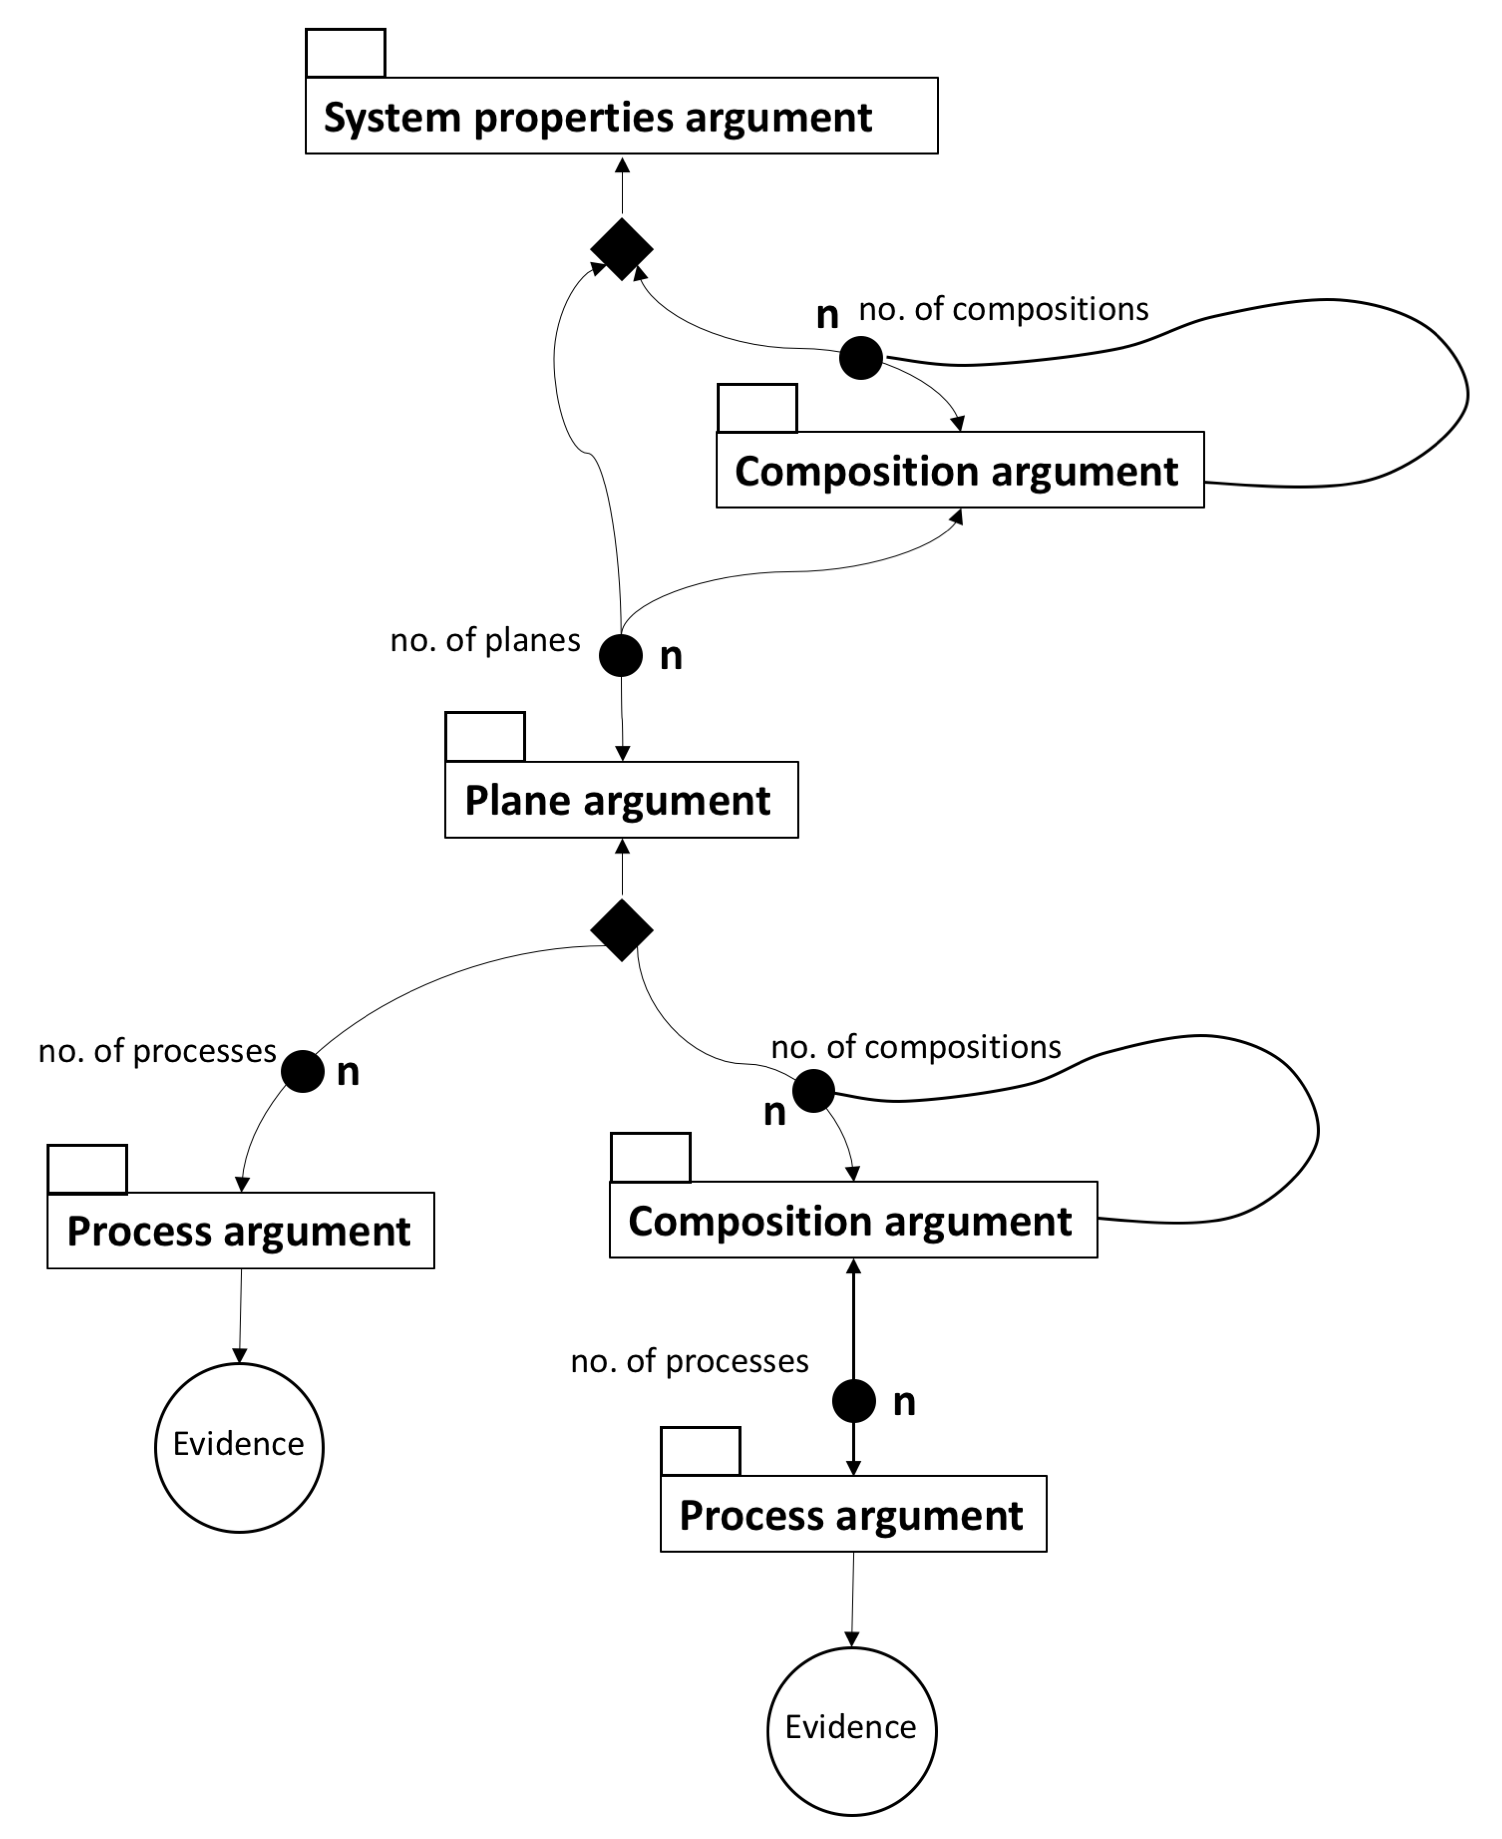
\includegraphics[width=.8\textwidth]{figures/modularassurancecase.png}
\caption{\label{fig:modularac} General modular assurance case structure for MILS systems}
\end{center}
\end{figure}
\clearpage

Figure~\ref{fig:modularac} comprises a general assurance case architecture for MILS systems, which has the potential to be applied to other systems than MILS systems as well. An assurance case structure specific to Adaptive MILS systems is illustrated in Figure~\ref{fig:modularac-adaptivemils} below. The structure is as follows: 
\begin{itemize}
\item{Adaptive MILS system}

\begin{itemize}
\item{Adaptive MILS Framework}

\begin{itemize}
\item{Monitoring plane}
\item{Adaptation plane}
\item{Configuration plane}
\item{Certification plane}
\item{Adaptive MILS platform (foundational plane)}

\begin{itemize}
\item{MILS Platform node(s)}
\begin{itemize}
\item{Separation Kernel (SK) instance(s)}
\item{MILS Network Subsystem (MNS) instance(s)}
\end{itemize}
\end{itemize}

\begin{itemize}
\item{Net (Deterministic Network)}
\begin{itemize}
\item{Physical network interfaces}
\item{Media}
\end{itemize}
\end{itemize}

\end{itemize}

\end{itemize}

\begin{itemize}
\item{System operational plane(s)}

\end{itemize}

\end{itemize}

The configuration of the various entities is contained within the respective assurance case argument patterns, as part of their local policy. The Adaptive MILS Platform configuration, which comprises the configuration of the MILS platform nodes, the global MNS configuration and the net configuration, is included as part of the foundational plane argument (in its security or safety policy) (Figure ~\ref{fig:foundational-plane}), or added in the context element to the goal elements within the assurance case argument (Section~\ref{sec:buildingblocks}). The same applies to the SK configuration and MNS configuration, which are part of the MILS platform node. Hence, the configuration may be thought of as iterated over the nodes, and is hierarchical (i.e. the node configuration is divided into SK instance configurations, MNS configurations, etc.). 
~\\
The goals of the SK instance(s) and MNS instance(s) support the MILS Platform Node(s) goal. The goal regarding MILS platform node(s) and the goal of the Net (Deterministic Network/TSN) together support the local policy of the Adaptive MILS platform. The various planes and the Adaptive MILS platform, collectively meet the Adaptive MILS framework goal, which supports the system properties argument. Accordingly, the local policies of the various planes together are required to be met in order to satisfy the security and/or safety policy of the Adaptive MILS system. Figure~\ref{fig:modularac-adaptivemils} provides an abstract overview, which is simplified for clarity and therefore does not include the specific components (i.e. the process argument patterns, comprising the evidence nodes, are not displayed in the image). 
\footnote{ The description in this section, as illustrated in Figure~\ref{fig:modularac-adaptivemils}, is entirely reflected in the System Properties argument pattern (Figure ~\ref{fig:systemproperties}), since this argument pattern is used to establish the "main", all-encompassing argument in the assurance case (i.e. all arguments originate from, or are encapsulated in, the System Properties argument pattern)}

\begin{figure}[htbp]
\begin{center}
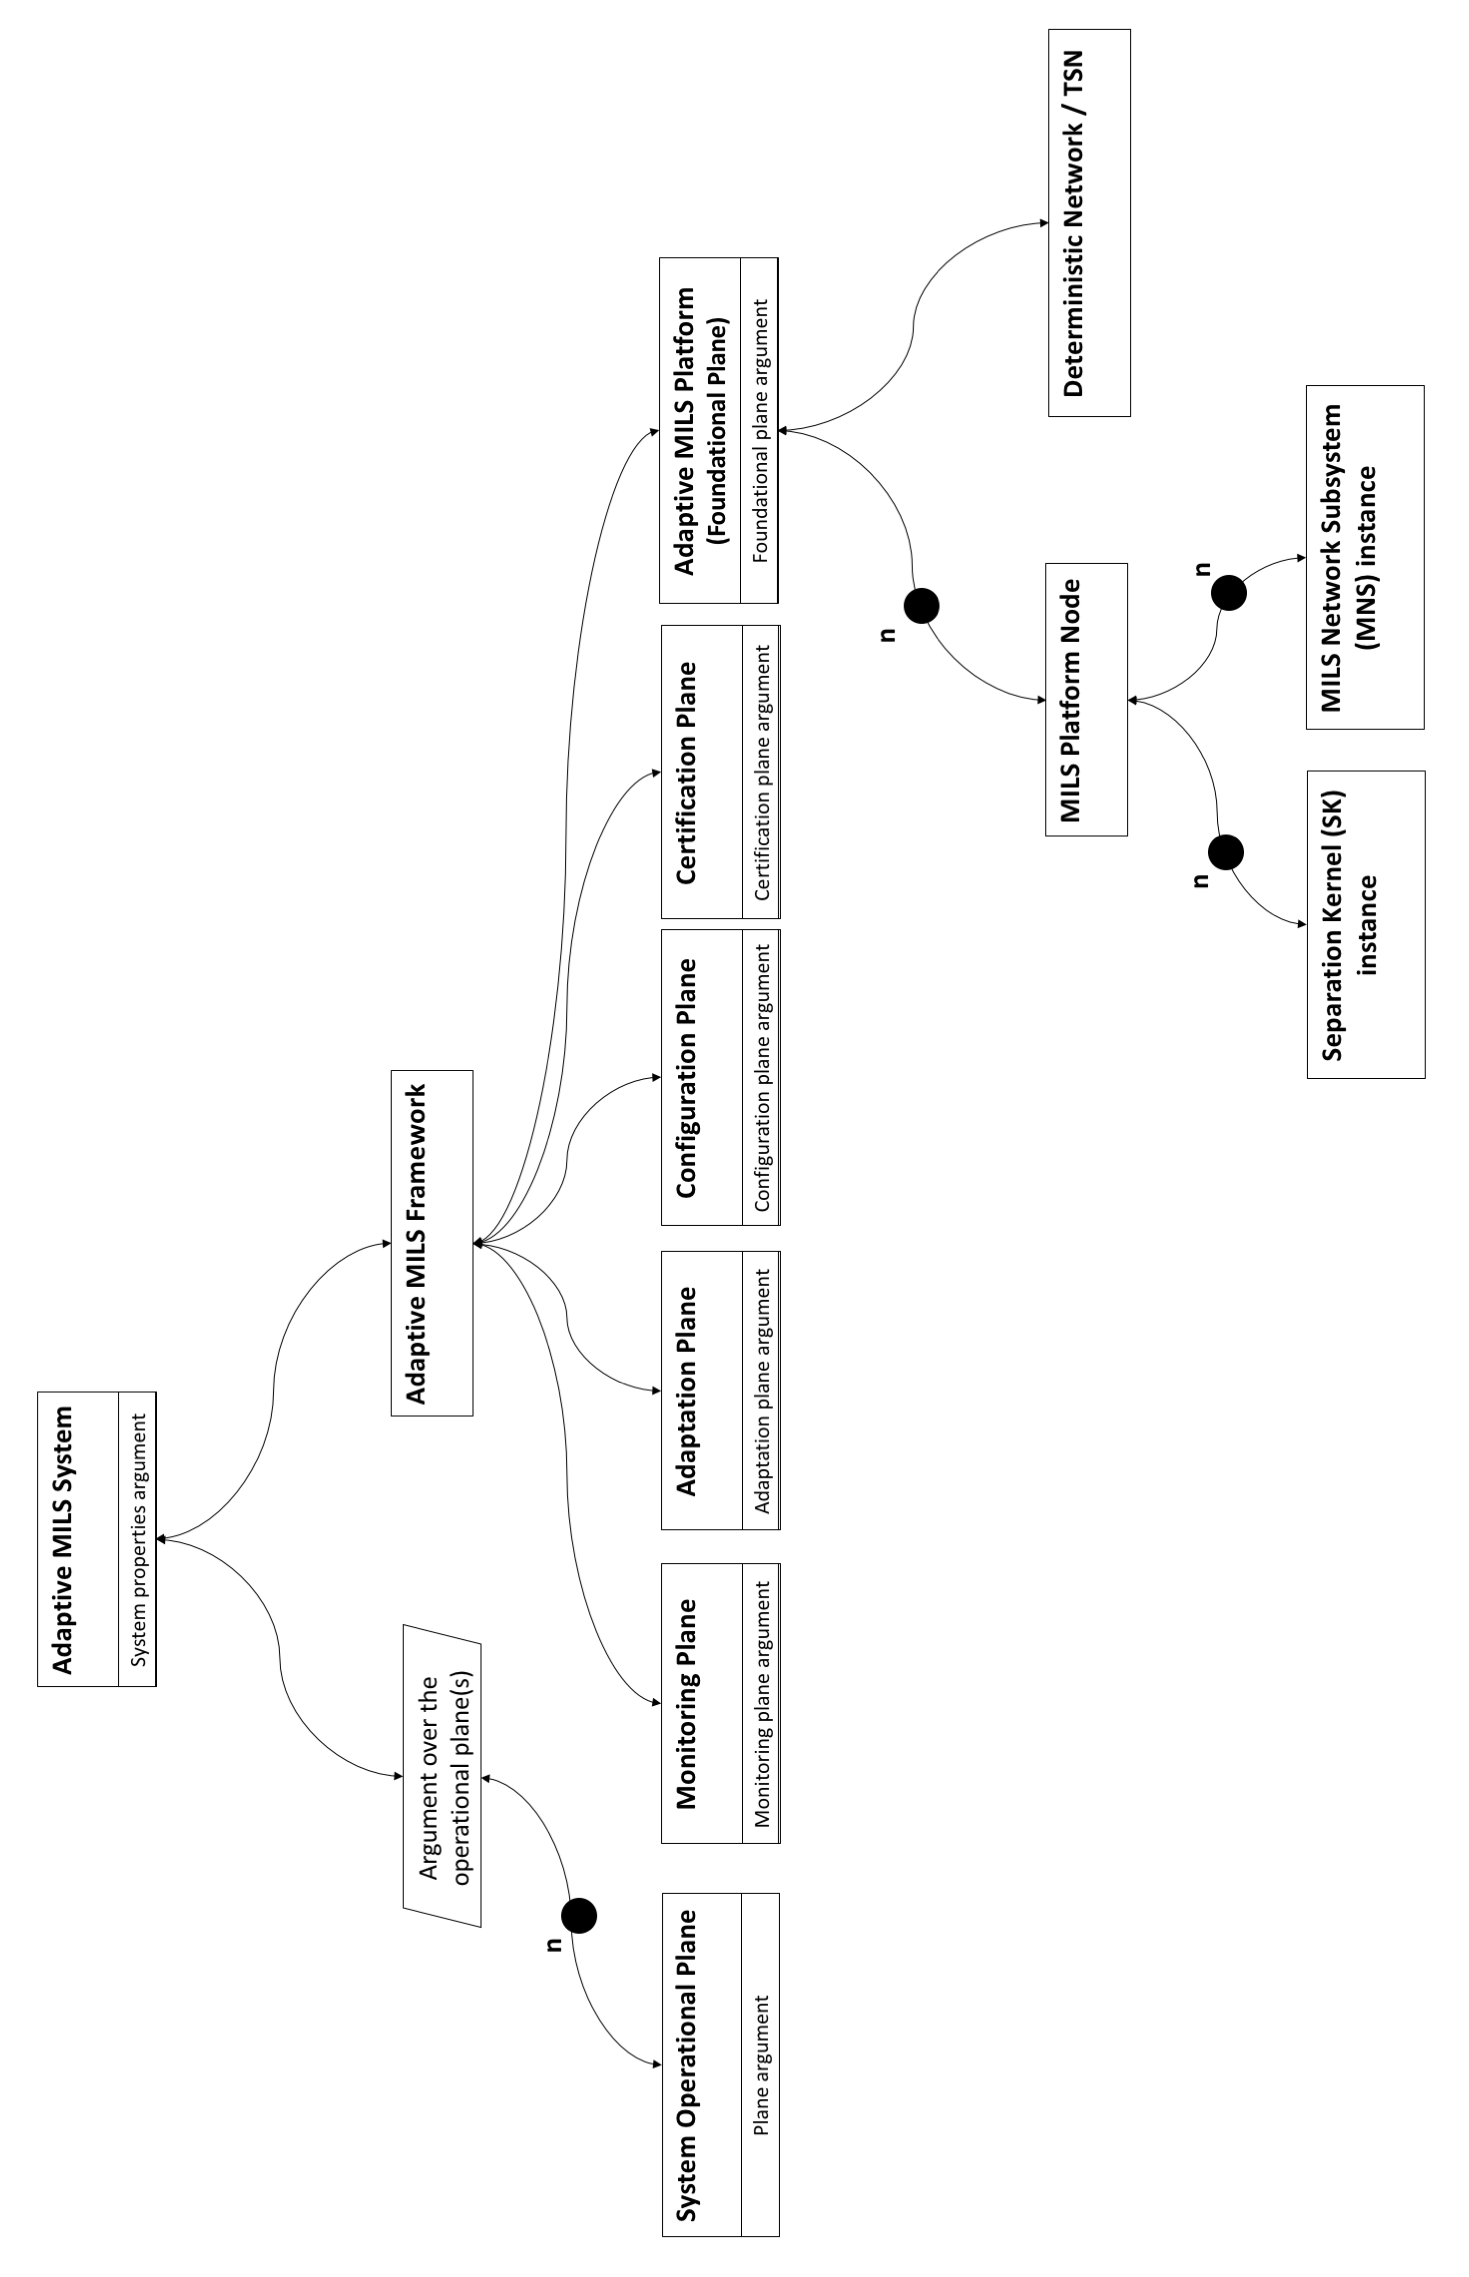
\includegraphics[width=.8\textwidth]{figures/modularassurancecase_adaptivemils2.png}
\caption{\label{fig:modularac-adaptivemils} Modular Assurance Cases of Adaptive MILS Systems}
\end{center}
\end{figure}
\clearpage


%%%%%%%%%%%%%%%%%%%%%%%%%%%%%%%%%%%%%%%%%%%%%%%%%%%%%%%%%%

\subsubsection{Hierarchy of Assurance Case Argument Patterns}
As a result of the self-adjusting nature of adaptive MILS systems and the structure of modular assurances, a hierarchy of assurance case argument patterns, that is different from the hierarchy of assurance cases of D-MILS systems, is proposed. D-MILS systems analyse and evaluate a system on the basis of a pre-defined offline system configuration, and therefore include both composition and implementation argument patterns. This approach is not deemed appropriate for adaptive MILS assurance cases, as it is more beneficial to evaluate the implementation against the generated evidence. Therefore, the implementation pattern is no longer included. Furthermore, trusted components are implemented as part of the process pattern. Figure~\ref{fig:hierarchy} encompasses the proposed hierarchy for assurance case argument patterns to build the adaptive MILS assurance case.\footnote{Although the planes that are part of the Adaptive MILS framework are to a large extent pre-defined, composition patterns have been included. This is due to the fact that these plane argument patterns still support the incorporation of all other argument patterns.} The composition pattern structure on the right side is an enlargement of the composition patterns illustrated on the left side. The patterns are designed to be as simple as possible, and have a single purpose. In accord, the patterns have high cohesion and allow for information hiding, thereby making it easier to instantiate and review the assurance case during evaluation. This structure allows for the reuse of patterns, the use of third-party components, and has the additional advantage that the argument and evidence regarding the behaviour of a component or composition of components can be made independently from the high-level security or safety policy.

\begin{figure}[htbp]
\begin{center}
\includegraphics[width=.8\textwidth]{figures/AdaptiveMILS-AC-Structure_2.png}
\caption{\label{fig:hierarchy} Assurance case argument pattern hierarchy for adaptive MILS systems}
\end{center}
\end{figure}

%%%%%%%%%%%%%%%%%%%%%%%%%%%%%%%%%%%%%%%%%%%%%%%%%%%%%%%%%%

\subsubsection{Overview of Assurance Case Argument Patterns}
The following is the set of patterns that can be employed to aid in the development of the assurance case of Adaptive MILS systems.

\begin{itemize}
\item System properties: Create an argument that the Adaptive MILS system enforces its required properties. These properties may regard security, safety, function and real-time properties.
\item Operational plane(s): create an argument about the compositional behaviour of the components and compositions of the operational plane
\item Adaptive MILS framework: since all planes in the Adaptive MILS framework are largely static, patterns for the various planes are established to create arguments specific to each of the planes to simplify instantiation and evaluation of the assurance case:
	\begin{itemize}
	\item Foundational plane (Adaptive MILS Platform): create an argument about complete data and processor time partitioning per processor and guarantee that only the connections as specified in the policy are established
	\item Monitoring plane: create an argument that the plane monitors and detects component failures such as malfunctioning or disruption of the communication network
	\item Adaptation plane: create an argument about the development of adaptation strategies in order to adapt to changing environmental conditions or dynamic repurposing of the system, while ensuring that adaptations preserve or recover vital overarching properties defined for the system
	\item Configuration plane: create an argument about dynamic reconfiguration capabilities
	\item Certification assurance plane: create an argument about AM-ETB tool integration and the verification and validation of results
	\end{itemize}
\item Interface: Create an argument that the communication between components or compositions in the architecture only occurs via connections explicitly defined in the CITADEL system model
\item Threats: Create an argument that threats are sufficiently mitigated
\item States and transitions: Create arguments that states and state transitions of components are in accordance with the states and transitions as specified in the CITADEL system model
\item Modes and transitions: Create arguments that modes and mode transitions of compositions are in accordance with the modes and transitions as specified in the CITADEL system model
\item Composition: Create arguments that formally defined properties of a system, as specified in the modelling language architecture description, are implemented and satisfied by an Adaptive MILS system.
\item Process: Create an argument for any component during the development, real-time adaptation and reconfiguration of an adaptive MILS system.
\item Tool: Create an argument about the trustworthiness of tools used as part of a process included in the assurance case. 
\item Person: Create an argument about the trustworthiness of people involved in a process included in the assurance case. 
\item Organisation: Create an argument about the trustworthiness of organisations involved in a process included in the assurance case.
\item Artefact: Create an argument about the trustworthiness of artefacts, either required by, or produced by, a process included in the assurance case.
\item Technique: Create an argument about the trustworthiness of techniques applied when performing as part of a process included in the assurance case.
\item Trusted software component: Create an argument about the correct implementation of trusted software components within a process.  
\end{itemize}

Furthermore, the AM-ETB should support the addition of supplementary (custom) assurance patterns, which are required to conform to the specification of Adaptive MILS assurance case argument patterns (see Section~\ref{sec:ap-rules}). In addition, it is important to note that the argument patterns are used as aid for the instantiation of the assurance case, and may be modified and are further defined upon instantiation. 

%%%%%%%%%%%%%%%%%%%%%%%%%%%%%%%%%%%%%%%%%%%%%%%%%%%%%%%%%%

\subsubsection{Structure and Specification of the Adaptive MILS Argument Pattern}\label{sec:ap-rules}
The following section describes the structure and specification of Adaptive MILS argument patterns, which should be considered when developing assurance cases based on the argument patterns, as well as when creating new argument patterns. 

\paragraph{Building Blocks}\label{sec:buildingblocks}~\\
Adaptive MILS systems employ the GSN (Goal Structuring Notation) notation for the development of assurance cases. GSN assurance cases are constructed and visualised by a set of GSN elements that collectively establish a goal structure. The GSN notation is used for the construction of Adaptive MILS assurance cases to allow for a comprehensible structure of documentation, and to ensure a clear mapping between evidence and claims in the arguments of the assurance case. 

The following GSN elements are included in Adaptive MILS assurance cases, and are largely taken from \cite{GSN_standard}:
	\begin{itemize}
	\item Goal: The goal element is employed to specify a claim 
	\item Undeveloped goal: An undeveloped goal element (a goal element with the hollow-diamond "undeveloped entity" symbol at the centre-bottom) presents a claim which is intentionally left undeveloped in the argument.
	\item Sub-goal: Goals can be broken into sub-goals, which may consist of safety or security requirements of the system, that together satisfy the claim. As such, a sub-goal in GSN represents a sub-claim. 
	\item Away goal: An away goal, as specified in \cite{GSN_standard}, "is rendered as a rectangle with a bisecting line in the lower half of the rectangle. The area in the lower portion contains a miniature shaded module symbol." An away goal indicates that the claim is represented in another argument in the assurance case.
	\item Evidence: The evidence element comprises the evidence to support the claims. All the evidence nodes in argument patterns are directly connected to their parent subgoals without intervening strategies.
	\item Strategy: The strategy element is utilised to make an argument about how sub-goals and evidence support the goals (claims). The kind of argument employed (for instance, an strategy over components or requirements) is written inside the strategy box. Strategies between a goal and its sub-goals are optional in the GSN notation. Simultaneously, it is also possible to include multiple strategies. 
	\item Assumption: The assumption element signifies the assumptions under which the system or design satisfies the claim(s). Providing assumptions is optional, but recommended to ensure the safety and security of an adaptive system. Assumptions can be used to support goals, sub-goals and strategies. 
	\item Justification: The justification element constitutes the justification of why the argument, sub-goals or evidence are appropriate to satisfy the claim: "Argument authors may feel the need to justify a particular claim or argument strategy, to provide some explanation as to why they consider it acceptable. This is achieved in GSN by the use of the justification element" \cite{GSN_standard}. Providing a justification for the application of a strategy is optional, and can be used to support goals, sub-goals and strategies. 
	\item Context: The context element is implemented to refer to CITADEL system models that specify the goals or local policies, or other requirements necessary to support the goal or sub-goal. According to \cite{Rushby15understanding-and-evaluating}, contexts provide "explications": that is "the text in a context element must be of the form X: Y where X is a phrase and Y is its explication. . . Y should identify relevant documentation where appropriate" \cite{GSN_standard}. Similar to assumptions and justifications, context elements can be connected to goals, sub-goals and strategies.
	\end{itemize}
The relationship between these building blocks in GSN defines predicate-conclusion relationships between goals and sub-goals, and designates how evidence provides support to the claims and the relationship between the argument and its context. Two types of arrowheads can be distinguished to designate relationships between the GSN elements: 
	\begin{itemize}
	\item Solid arrowhead: The solid arrowhead signifies \textit{"SupportedBy"}, referring to the inferential or evidential relationships between elements.
	\item Open arrowhead: The open arrowhead signifies \textit{"InContextOf"}, indicating contextual relationships \cite{GSN_standard}.
	\end{itemize}


\paragraph{Claims and Identification of Requirements}
~\\
Assurance cases make claims to demonstrate that a system is safe or secure. Claims of adaptive systems encompass high-level abstract descriptions of the mission of the system, or part of the system, based on which detailed requirements are derived. 
%The security claims made in Adaptive MILS systems are demonstrably satisfied through requirements and their supported evidence.  As the initial system design may be abstract and incomplete, so will be the assurance case, and the initial claims and arguments may be fuzzy and incomplete. Therefore, a standards-based method of instantiation facilitates the specification of claims, as well as the requirements and evidence to support the claims, depending on type of system (Section~\ref{sec:standards-based-method}). 
Three types of requirements, as described in the section below, should be considered when defining the necessary requirements as part of the argument patterns (in case a standards-based approach cannot be applied), and for the instantiation and further development of assurance cases. Whenever the assurance case is instantiated automatically, based on the assurance case argument patterns (see Section~\ref{sec:automated-instantiation}), the requirements to support the claims should be specified in the system model (or another manner that enables the automated instantiation of the assurance case). These requirements are then incorporated in the assurance case by connecting context elements to goals, sub-goals or strategies. 

The following types of requirements can be distinguished:
\begin{itemize}
\item \textbf{Requirements to satisfy security properties of an Adaptive MILS system}

The security properties of an Adaptive MILS system concern the CIA (confidentiality, integrity and availability) security properties that apply in the general context of the processing, storage, and communication of data and the provision of services. The security properties are generally extended by additionally considering authentication, non-repudiation and authorisation \cite{Lipson13evidence-of-assurance}. 
\end{itemize}


Even though the requirements to satisfy security properties are capable of fulfilling high-level claims and thereby demonstrate the system is secure, "an observed absence of security incidents might not be evidence of robust security, but instead, could be an indication of the inability of the system to detect attacks, such as lack of logging, failure to regularly audit existing logs, or protecting/isolating logs from erasure or modification by an attacker" \cite{Lipson13evidence-of-assurance}. In addition, a system may be insecure even without active attackers, as a system will not be able to detect the action of passive capturing (i.e. side channels pose difficulties for the system itself to detect it is under attack). Therefore, it is just as important for adaptive systems to demonstrate what it means for the system to be unsafe, or insecure, and how to counter such an insecure state of the system. The following requirements regard the consideration of unsafe states of a system:
\begin{itemize}
\item \textbf{Requirements to ensure absence of vulnerabilities}
 
These requirements concern the absence of vulnerabilities (in the design or implementation) that could be exploited to break the system's security model. "Vulnerabilities arise when assumptions about the (threat) environment in which a system operates are incorrect or incomplete or when presumed constraints on the behaviour of a potential adversary do not reflect reality"  \cite{Lipson13evidence-of-assurance}. In addition, vulnerabilities that show no indication that the system may be attacked need to be considered. In accord, threats assurance case argument patterns can be included as part of the assurance case of Adaptive MILS systems to enable evaluation of enforcement of requirements to demonstrate the absence of vulnerabilities.  

~\\
\item \textbf{Requirements to ensure cyber resilience}

Cyber resilience involves a combination of computer security and organisation risk management: "an organisation that has resilient operations should be able to systematically and transparently cope with disruptive events so that the overall ability of the organisation to meet its mission is minimally or not adversely affected" \cite{Lipson13evidence-of-assurance}. According to \cite{Lipson13evidence-of-assurance}, claims made to ensure the cyber resilience of a system may be satisfied through three sets of requirements: resistance to attack or other stress; recognition of a survivability problem or crisis and its effect on the system; and recovery, the ability to restore services after an attack or other crisis. The claim of cyber resilience is met by showing that the residual risk has been reduced to as low as reasonably practicable (a principle known as "ALARP").
Requirements to ensure the cyber resilience of Adaptive MILS systems are, for instance, included in the sub-goal regarding dynamic risk assessment (based on context-awareness), as part of the assurance case argument pattern of the adaptation plane. 
In the process of restoring services after a crisis, the system may not comply to the assurance arguments specified before the crisis. Using arrays of acceptable values of attributes in security (and safety) properties, as opposed to single values, has the potential to ensure the system remains compliant to the arguments. If the required modifications to the system after crisis are highly transformative, the use of an updated system model established by the configuration plane is required. 
\end{itemize}


\paragraph{Specification of Evidence}\label{sec:specificationofevidence}
~\\
Even though persuasive argumentation and a strong, comprehensive set of requirements plays a major role in satisfying the claims of an assurance case, the strength of the arguments and of the assurance case as a whole depends on the quality and completeness of the evidence to support high-assurance claims of security or safety. 

A standards-based methodology can provide assistance by indicating necessary pieces of evidence, to support particular requirements and claims, early in the development process. A third-party expert, such as a certifier or auditor, may additionally assist in reviewing the assurance case argument patterns to decide what evidence should be included. This approach yields the additional advantage that the selected body of evidence is in line with the evidence required by evaluators that evaluate the assurance case, and is increasingly likely to follow the standards necessary for certification.

The evidence of an assurance case may validate and verify the requirements through various types of evidence generation, such as testing (i.e. environmental testing, unit testing, system testing, fuzzing, etc), formal methods (i.e. model checkers, theorem provers, etc), simulations, audits, and review of artefacts such as design and guidance documents, and life cycle processes. "As such, it is a cue to the development team that when the life cycle development processes generate artefacts that can serve as evidence (i.e. requirements documents, design rationale, test plans, test results, and results of code reviews), the artefacts should be preserved for use in an assurance case" \cite{Lipson13evidence-of-assurance}. Depending on the component and type of evidence, it may be possible to generate the evidence automatically. If this is not possible, evidence to support the assurance arguments should be generated manually, through testing or other types of reviews. The different manners of generating evidence and their limitations as specified in \cite{Hawkins12framework-sufficiency} should be considered when selecting appropriate types of evidence to support goals or sub-goals. 

It is essential that each claim in an assurance case should eventually end with an evidence node. However, this does not necessarily mean that each assurance case argument pattern should end with an evidence node. The pattern could, for instance, also be supported by other argument patterns that end with evidence nodes. For instance, the process argument pattern for Adaptive MILS systems should always end with evidence nodes, and therefore supports abundant other Adaptive MILS argument patterns. This can be either only from the process argument itself, or provided by properties arguments (tool, person, organisation, artefact, technique) supporting the process argument. 

In case there are multiple ways to demonstrate satisfaction of goals (i.e. based on different processes), the approach with the most convincing strategy and evidence is to be chosen. 

\paragraph{Specification of Assumptions}
~\\
The evidence to substantiate the claims made in an assurance case should not only consider the system itself, but should additionally take into account the operational environment of the system. Considering the environment, and the risks these pose on the system, is especially important in cases where the evidence supports claims regarding the resilience of the system. "For example, determining whether the security risks to the system's mission have been reduced to as low as reasonably practicable (ALARP) cannot be accomplished by considering (e.g., analysing or observing) the system's security mechanisms solely in isolation" \cite{Lipson13evidence-of-assurance}. Therefore, the operational environment of the system should either be considered and included as part of the evidence, or incorporated as environmental assumptions. 

Hence, it is necessary to specify assumptions under which the system or design satisfies the claims. Realistically, assumptions are to be specified and reviewed manually. \cite{Lipson13evidence-of-assurance} provides insight into what environmental aspects and other, more general, aspects may be included in the assumptions. However, as Rushby states, "mechanised tools such as theorem provers and model checkers can analyse theorems of this form and provide an inestimable benefit by helping to identify necessary assumptions" \cite{Rushby09asafety-case}. These mechanised tools could be provided by the AM-ETB to identify necessary assumptions, yet manual review and refinement of assumptions remains a requirement. 

\paragraph{Compatibility with System Model}\label{sec:languagemodelcompatibility}
~\\
Assurance case argument patterns for MILS systems are required to be (largely) compatible with the system models.
In the case of Adaptive MILS the system models are defined in the CITADEL Modelling and Specification Language  \cite{CITADEL-D3.1}, thereby enabling automatic instantiation of the argument patterns (see Section ~\ref{sec:automated-instantiation}). It is therefore essential that the pattern description specifies what information should be taken from the CITADEL system model to instantiate the argument pattern.  


\paragraph{Information Hiding}\label{sec:infohiding}
~\\
The argument pattern should have high cohesion and allow for information hiding, thereby simplifying the automatic instantiation, development and evaluation of the assurance case. 

\paragraph{Adding New Assurance Case Argument Patterns}
~\\
New assurance case argument patterns for Adaptive MILS systems should only be created if no similar Adaptive MILS argument patterns exist, and should take into account the information described in Section~\ref{sec:ap-rules}, Section~\ref{sec:languagemodelcompatibility} and Section~\ref{sec:infohiding}.


%%%%%%%%%%%%%%%%%%%%%%%%%%%%%%%%%%%%%%%%%%%%%%%%%%%%%%%%%%

\subsubsection{Adaptive MILS Assurance Case Argument Patterns}
This section describes the various assurance argument patterns in more detail. The principal patterns from the top-level assurance view are the system properties argument pattern and the process and composition patterns that are used to support the system properties arguments.
However, we start by introducing the CITADEL Framework and the argument patterns for the planes of the Framework as these support all of the higher-level process, property and composition arguments.
Subsequently, the argument patterns of the different properties of process patterns are defined. For each of the argument patterns presented, an indication is provided of the information required from the formal system model to instantiate the argument pattern. 

%%%%%%%%%%%%%%%%%%%%%%%%%%%%%%%%%%%%%%%%%%%%%%%%%%%%%%%%%%

\paragraph{Argument Patterns for the Adaptive MILS Planes}
~\\

Architectural entities referred to as \emph{planes} comprise the \emph{CITADEL Framework}, shown in Figure~\ref{fig:citadel-fw}, within which an Adaptive MILS system is constructed. 
\begin{figure}[htbp]
\begin{center}
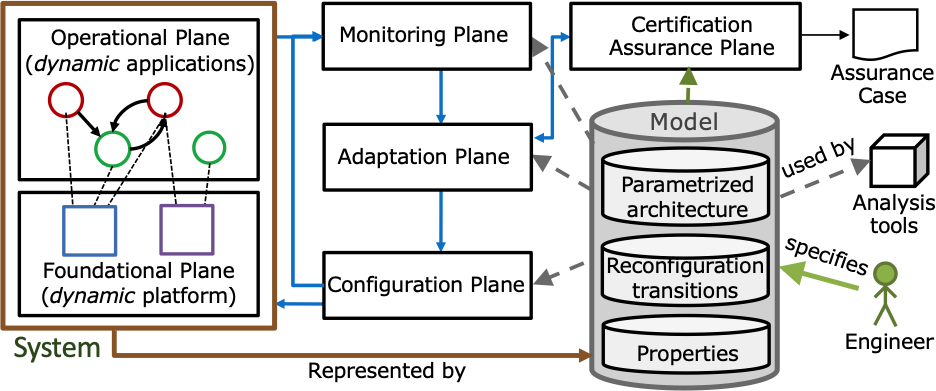
\includegraphics[width=.8\textwidth]{figures/citadel-fw.pdf}
\caption{\label{fig:citadel-fw} CITADEL Framework}
\end{center}
\end{figure}
Each plane can include one or multiple components, or one or several hierarchical compositions of components. The goal of a plane is satisfied when the compositional behaviour of the compositions and/or components comprising that plane meet their local policies, as well as ensure that the interaction between them is as specified in the top level policy, which can be demonstrated through the interface argument.

The model of a dynamically reconfigurable distributed MILS system, though it is described in terms that have specific interpretations in the context of MILS, is quite general and can be applied to other kinds of modular, configurable distributed systems in a more familiar way when a suitable substitution of terms is applied.
The most important terms to address are those that relate to the concrete system itself (labeled ``System'' in the figure).
More conventionally, the ``operational plane(s)'' might be referred to in a more familiar way as ``application [plane](s)'' and the
``foundational plane'' as the ``platform [plane]''.

Some systems, however, do not require use of all the the conceptual planes of the CITADEL Framework.
For example, a statically configured system (one that is configured once on installation or on startup) does not need an adaptation plane.
It may not need a monitoring plane, or it may have one to trigger mode changes or detect and respond to other foreseeable runtime conditions.
Its configuration plane degenerates to an offline configuration tool or procedure, and its certification assurance plane degenerates to offline assurance activities.
For many systems the certification assurance plane'' does not require the level of rigor of modelling and verification that is assumed for MILS.
Other examples can be imagined for systems that are standalone (not distributed over a network) or which have a fixed set of applications that do not change during an execution session.
~\\
~\\
\clearpage
\emph{Operational plane}

An operational plane is an application plane of an Adaptive MILS system, and is the least pre-defined plane
\emph{a priori}, as the components included in the operational plane depend on the purpose of the Adaptive MILS system (not a general-purpose system). Therefore, a generic argument pattern is designed for the operational plane, which can be further developed manually, depending on the safety and security goals of the application (Figure ~\ref{fig:operational-plane}).

\begin{figure}[htbp]
\begin{center}
\includegraphics[width=.8\textwidth]{figures/patterns/operationalplane.pdf}
\caption{\label{fig:operational-plane} Operational plane argument pattern}
\end{center}
\end{figure}

\textbf{Related patterns}
The argument created from this pattern supports the arguments created using the system properties argument pattern.

\textbf{Pattern instantiation}
The information required for the parameters of the operational plane argument pattern are described in Table ~\ref{tab:op_plane_params}.

\begin{table}[htbp]
    \centering
    \caption{Operational plane pattern parameters}
    \begin{tabularx}{\textwidth}{| l | X | X |}
        \hline
        \textit{\textbf{Parameter}}     & \textit{\textbf{Description}}    & \textit{\textbf{Source}}     \\ \hline
        Plane        & Name of the plane      & Plane name in CITADEL system model (i.e. "citadel-framework.aadl"); \textit{ComponentImplementation}         \\ \hline
        Local policy        & Local policy of the plane      & Implementation description in CITADEL system model describing \textit{ComponentImplementation}        \\ \hline
        Parameters       & The architecture is specified using parameters; different static architectures can be instantiated by specifying the values of the parameters      & ComponentImplementation: [\textbf{parameters} \textit{Parameters}]        \\ \hline
        Assumptions       & Assumptions on the parameters & ComponentImplementation: [\textbf{assumptions} \textit{ParameterAssumptions}]        \\ \hline
        Components       & The components of the plane & ComponentImplementation: [\textbf{subcomponents} \textit{Subcomponents}]         \\ \hline
        Properties       & Properties that are used to specify temporal formulas, contracts, and other constructs that change the semantics of the CITADEL Model & ComponentType: [\textit{Properties}]        \\ \hline
    \end{tabularx}
    \label{tab:op_plane_params}
\end{table}

\clearpage
\emph{Foundational plane}

The concept of the MILS foundational plane,
along with the other plane designations,
emerged during the CITADEL project.
The foundational plane is also referred to as the \emph{MILS platform}.
Depending on the context it can refer to a single stand-alone system or a MILS network of such systems (nodes) by the inclusion of a MILS networking component in each system.
In the case of a MILS network, the complete hardware and the resource management system software, including those implementing the network, are considered to comprise the MILS platform.
These concepts of how components of the MILS platform could be integrated with assurance under an appropriate set of assumptions and standards were elaborated initially in the MILS Integration Protection Profile (MIPP) \cite {MIPP} and its accompanying commentary
\cite{MIPP-commentary}, and later evolved into a MILS Platform Protection Profile (MPPP) \cite {MPPP} and its accompanying commentary \cite{MPPP-commentary}.

The foundational plane includes various foundation element components; the platform node(s), containing separation kernel instances and MILS Network Subsystem (MNS) instances, and the TSN (Time Sensitive Network) \cite{TSN}\footnote{In the D-MILS project the network technology was Time-Triggered Ethernet (TTE), which evolved into Time Sensitive Network (TSN), an industry standard, for the CITADEL project.}. The separation kernel instances enable the system to run applications of diverse security domains on the same processor. TSN maintains synchronised time in the Adaptive MILS system, and ensures that critical information is delivered timely and additionally optimises bandwidth by labelling messages with different levels of priority. Hence, it enhances communication over the Adaptive MILS system by taking into account that applications of mixed time criticality share a single network. 
The separation kernel makes an argument to ensure complete data and processor time partitioning per processor, and provides role-based and capabilities-based access control to resources and exported interfaces. In addition, the separation kernel provides configuration introspection primitives that permit an authorised subject to obtain a representation of the current configuration. The evidence to substantiate the subgoals of the argument comprise a CC evaluation that is compliant to the EURO-MILS protection profile \cite{EMPP}. 
Moreover, the foundational plane includes a Network Scheduling Master (NSM), which monitors and adapts the network when configuration change is necessary (Figure ~\ref{fig:foundational-plane}).

\begin{figure}[htbp]
\begin{center}
%\includegraphics[scale=0.5,width=\textwidth,height=\textheight,keepaspectratio]{figures/patterns/foundationalplane3.pdf}
\includegraphics[height=\textheight,keepaspectratio]{figures/patterns/foundationalplane3.pdf}
\caption{\label{fig:foundational-plane}Foundational plane argument pattern}
\end{center}
\end{figure}

\textbf{Related patterns}
The argument created from this pattern supports the arguments created using the system properties argument pattern.

\textbf{Pattern instantiation}
The information required for the parameters of the foundational plane argument pattern are described in Table ~\ref{tab:found_plane_params}.

\begin{table}[htbp]
    \centering
    \caption{Foundational plane pattern parameters}
    \begin{tabularx}{\textwidth}{| X | X | X |}
        \hline
        \textit{\textbf{Parameter}}     & \textit{\textbf{Description}}    & \textit{\textbf{Source}}     \\ \hline
        Plane        & Name of the plane      & Plane name in CITADEL system model (i.e. "citadel-framework.aadl"); \textit{ComponentImplementation}         \\ \hline
        Local policy        & Local policy of the plane      & Implementation description in CITADEL system model describing \textit{ComponentImplementation}        \\ \hline
        Parameters       & The architecture is specified using parameters; different static architectures can be instantiated by specifying the values of the parameters      & ComponentImplementation: [\textbf{parameters} \textit{Parameters}]        \\ \hline
        Assumptions       & Assumptions on the parameters & ComponentImplementation: [\textbf{assumptions} \textit{ParameterAssumptions}]        \\ \hline
        Components       & The components of the plane & ComponentImplementation: [\textbf{subcomponents} \textit{Subcomponents}]         \\ \hline
        Properties       & Properties that are used to specify temporal formulas, contracts, and other constructs that change the semantics of the CITADEL Model & ComponentType: [\textit{Properties}]        \\ \hline
         Results of network fault propagation analysis        & reference to the results of the fault propagation analysis      & Manual         \\ \hline
    \end{tabularx}
    \label{tab:found_plane_params}
\end{table}

\clearpage
\emph{Monitoring plane}

The monitoring plane employs run-time monitors to detect component failures such as malfunctioning or disruption of the communication network. The monitoring framework supports state monitoring and communication monitoring (Figure ~\ref{fig:monitoring-plane}).

\begin{figure}[htbp]
\begin{center}
\includegraphics[width=.8\textwidth]{figures/patterns/monitoringplane.pdf}
\caption{\label{fig:monitoring-plane} Monitoring plane argument pattern}
\end{center}
\end{figure}

\textbf{Related patterns}
The argument created from this pattern supports the arguments created using the system properties argument pattern.

\textbf{Pattern instantiation}
The information required for the parameters of the monitoring plane argument pattern are described in Table ~\ref{tab:mon_plane_params}.

\begin{table}[htbp]
    \centering
    \caption{Monitoring plane pattern parameters}
    \begin{tabularx}{\textwidth}{| l | X | X |}
        \hline
        \textit{\textbf{Parameter}}     & \textit{\textbf{Description}}    & \textit{\textbf{Source}}     \\ \hline
        Plane        & Name of the plane      & Plane name in CITADEL system model (i.e. "citadel-framework.aadl"); \textit{ComponentImplementation}         \\ \hline
        Local policy        & Local policy of the plane      & Implementation description in CITADEL system model describing \textit{ComponentImplementation}        \\ \hline
        Parameters       & The architecture is specified using parameters; different static architectures can be instantiated by specifying the values of the parameters      & ComponentImplementation: [\textbf{parameters} \textit{Parameters}]        \\ \hline
        Assumptions       & Assumptions on the parameters & ComponentImplementation: [\textbf{assumptions} \textit{ParameterAssumptions}]        \\ \hline
        Components       & The components of the plane & ComponentImplementation: [\textbf{subcomponents} \textit{Subcomponents}]         \\ \hline
        Properties       & Properties that are used to specify temporal formulas, contracts, and other constructs that change the semantics of the CITADEL Model & ComponentType: [\textit{Properties}]        \\ \hline
    \end{tabularx}
    \label{tab:mon_plane_params}
\end{table}

\clearpage
\emph{Adaptation plane}

The adaptation plane synthesises the target architecture of the system while ensuring that adaptations preserve vital overarching properties defined for the system. The adaptation plane makes use of various agents:
\begin{itemize}
\item A verification agent invoked by the adaptation control system that uses the online verification framework to verify properties of a proposed new configuration and of reconfiguration plans to achieve the new configuration
\item A just-in-time-certification agent that assembles and records the derivation of evidence that a new configuration and the transition to the new configuration will satisfy certification requirements
\end{itemize}

It is important that assurance cases of Adaptive MILS systems do not only specify the requirements of what it means for the system to be secure, since this may introduce the notion of \textit{confirmation bias}. Rather, the opposite goal must also be considered; to demonstrate that the system is unsafe, or insecure. This could be achieved by employing threat arguments (see Section~\ref{sec:threats-ap}), or by demonstrably considering risk. Accordingly, the dynamic risk assessment argument pattern aims to continuously demonstrate that major threats to the system and its environment are identified, and by subsequently determining appropriate adaptations in such contexts during the process of developing the adaptation strategy (Figure ~\ref{fig:adaptation-plane}). 

The concept of dynamic risk assessment is to enable the adaptive system to perceive and interpret risk factors. The adaptation plane should be able to assess the risk of the situation or context before determining how the system should adapt, thereby being capable of selecting safe reconfigurations and avoiding reconfigurations that could lead to incorrect or insecure functioning of the system. Thus, the security of the system is assured by complex mechanism(s) that select the best adaptation in any given context. For certain scenarios requiring dynamic risk assessment, a context-awareness or situation awareness model may be employed, which provides a means to recognise situation attributes that are relevant for the security and correct functioning of the system. Hence, the model should be capable of perceiving the system's context, identifying possible adaptations and predicting their results (whether they might lead to a crisis or not), by taking into account changes in the environment and behaviour of other components within the system. Subsequently, in an attempt to avoid (similar) critical situations after a crisis, a root-cause analysis should be included as part of dynamic risk assessment. 

The following are the main requirements for the context-awareness model, which should be included as part of the context or as an assumption of the argument \cite{Wardzinski08safety-arguments}.
\begin{itemize}
\item The model should recognise contexts that are relevant for system safety and security (including safe, hazardous contexts and accidents)
\item Attributes that are used to identify and classify contexts should be capable of being measured with the use of sensors, or their values should be deducible from an accessible information source
\item The model gives information regarding the potential adaptations of the current situation
\item The model can predict and assess the safety or security of a situation as a result of a given action or action scenario. The prediction should take into account the behaviour of other components, systems and events in the environment. 
\item The model should be capable of representing incomplete or uncertain data, which may lead to uncertain risk assessment. The model should preserve safety and security when the risk assessment results are uncertain. The loss of context awareness (when the control system is not able to assess the situation) is interpreted as an unsafe context or situation.
\item The depth of predictions of future contexts is sufficient with regards to ensuring avoidance of unsafe states. Thus, the system has enough time to avoid critical situations, after perceiving risks in the current context. 
\item The model implementation is effective within required time limits. 
\end{itemize}

The adaptation plane pattern is shown in Figure ~\ref{fig:adaptation-plane}, which is further supported by the context awareness requirements shown in Figure ~\ref{fig:context-adaptation-plane} as a continuation of the adaptation plane pattern.

\begin{figure}[htbp]
\begin{center}
\includegraphics[scale=0.8,width=.8\textwidth]{figures/patterns/adaptationplane4-1.pdf}
\caption{\label{fig:adaptation-plane} Adaptation plane argument pattern}
\end{center}
\end{figure}

\begin{figure}[htbp]
\begin{center}
\includegraphics[scale=0.4,width=\textwidth,height=\textheight,keepaspectratio]{figures/patterns/adaptationplane4-2.pdf}
\caption{\label{fig:context-adaptation-plane} Context awareness supporting adaptation plane pattern}
\end{center}
\end{figure}

\textbf{Related patterns}
The argument created from this pattern supports the arguments created using the system properties argument pattern.

\textbf{Pattern instantiation}
The information required for the parameters of the adaptation plane argument pattern are described in Table ~\ref{tab:adapt_plane_params}.

\begin{table}[htbp]
    \centering
    \caption{Adaptation plane pattern parameters}
    \begin{tabularx}{\textwidth}{| X | X | X |}
        \hline
        \textit{\textbf{Parameter}}     & \textit{\textbf{Description}}    & \textit{\textbf{Source}}     \\ \hline
        Plane        & Name of the plane      & Plane name in CITADEL system model (i.e. "citadel-framework.aadl"); \textit{ComponentImplementation}         \\ \hline
        Local policy        & Local policy of the plane      & Implementation description in CITADEL system model describing \textit{ComponentImplementation}        \\ \hline
        Parameters       & The architecture is specified using parameters; different static architectures can be instantiated by specifying the values of the parameters      & ComponentImplementation: [\textbf{parameters} \textit{Parameters}]        \\ \hline
        Assumptions       & Assumptions on the parameters & ComponentImplementation: [\textbf{assumptions} \textit{ParameterAssumptions}]        \\ \hline
        Components       & The components of the plane & ComponentImplementation: [\textbf{subcomponents} \textit{Subcomponents}]         \\ \hline
        Properties       & Properties that are used to specify temporal formulas, contracts, and other constructs that change the semantics of the CITADEL Model & ComponentType: [\textit{Properties}]        \\ \hline
        Context        & Indicates what the context of the dynamicRiskAnalysis argument is & manual     \\ \hline
    \end{tabularx}
    \label{tab:adapt_plane_params}
\end{table}

\clearpage
\emph{Configuration plane}

The configuration plane is a combination of offline functions and online functions that provide dynamic reconfiguration capabilities. The configuration plane constitutes a configuration state controller, a platform reconfiguration planner and an Adaptive MILS Platform Configuration Compiler (MPCC). 

The configuration plane develops a reconfiguration plan, and mediates the use of the dynamic reconfiguration primitives of the separation kernel and the network by enforcing adaptation policies on proposed reconfiguration plans (Figure ~\ref{fig:configuration-plane}).

The configuration plane employs various agents:
\begin{itemize}
\item A configuration change agent provides a standard interface for dynamic reconfiguration of multiple components of the Adaptive MILS system, and can impose constraints, possibly with the assistance of a policy component, on the configuration change requests that it will issue to the separation kernel and other MILS platform components. 
\item A configuration state controller that invokes the dynamic reconfiguration primitives of the separation kernel and the network after a reconfiguration plan is approved.

\end{itemize}

\begin{figure}[htbp]
\begin{center}
\includegraphics[width=.8\textwidth]{figures/patterns/configurationplane2.pdf}
\caption{\label{fig:configuration-plane} Configuration plane argument pattern}
\end{center}
\end{figure}

\textbf{Related patterns}
The argument created from this pattern supports the arguments created using the system properties argument pattern.

\textbf{Pattern instantiation}
The information required for the parameters of the adaptation plane argument pattern are described in Table ~\ref{tab:config_plane_params}.

\begin{table}[htbp]
    \centering
    \caption{Configuration plane pattern parameters}
    \begin{tabularx}{\textwidth}{| X | X | X |}
        \hline
        \textit{\textbf{Parameter}}     & \textit{\textbf{Description}}    & \textit{\textbf{Source}}     \\ \hline
        Plane        & Name of the plane      & Plane name in CITADEL system model (i.e. "citadel-framework.aadl"); \textit{ComponentImplementation}         \\ \hline
        Local policy        & Local policy of the plane      & Implementation description in CITADEL system model describing \textit{ComponentImplementation}        \\ \hline
        Parameters       & The architecture is specified using parameters; different static architectures can be instantiated by specifying the values of the parameters      & ComponentImplementation: [\textbf{parameters} \textit{Parameters}]        \\ \hline
        Assumptions       & Assumptions on the parameters & ComponentImplementation: [\textbf{assumptions} \textit{ParameterAssumptions}]        \\ \hline
        Components       & The components of the plane & ComponentImplementation: [\textbf{subcomponents} \textit{Subcomponents}]         \\ \hline
        Properties       & Properties that are used to specify temporal formulas, contracts, and other constructs that change the semantics of the CITADEL Model & ComponentType: [\textit{Properties}]        \\ \hline
    \end{tabularx}
    \label{tab:config_plane_params}
\end{table}

\clearpage
\emph{Certification assurance plane}

The certification assurance plane comprises the AM-ETB, which enables tool integration, as well as the verification and validation of results. The AM-ETB encompasses different techniques and mechanisms to generate and manage the evidence needed for certification during system operation. The AM-ETB provides a framework for propagating system-level and inter-component constraints, enforcing standards, checking consistency, and providing automated review of evidence as a proxy for certification experts (Figure ~\ref{fig:certificationassurance-plane}). 

\begin{figure}[htbp]
\begin{center}
\includegraphics[width=.8\textwidth]{figures/patterns/certificationassuranceplane.pdf}
\caption{\label{fig:certificationassurance-plane} Certification assurance plane argument pattern}
\end{center}
\end{figure}

\textbf{Related patterns}
The argument created from this pattern supports the arguments created using the system properties argument pattern.

\textbf{Pattern instantiation}
The information required for the parameters of the adaptation plane argument pattern are described in Table ~\ref{tab:cert_plane_params}.

\begin{table}[htbp]
    \centering
    \caption{Certification assurance plane pattern parameters}
    \begin{tabularx}{\textwidth}{| X | X | X |}
        \hline
        \textit{\textbf{Parameter}}     & \textit{\textbf{Description}}    & \textit{\textbf{Source}}     \\ \hline
        Plane        & Name of the plane      & Plane name in CITADEL system model (i.e. "citadel-framework.aadl"); \textit{ComponentImplementation}         \\ \hline
        Local policy        & Local policy of the plane      & Implementation description in CITADEL system model describing \textit{ComponentImplementation}        \\ \hline
        Parameters       & The architecture is specified using parameters; different static architectures can be instantiated by specifying the values of the parameters      & ComponentImplementation: [\textbf{parameters} \textit{Parameters}]        \\ \hline
        Assumptions       & Assumptions on the parameters & ComponentImplementation: [\textbf{assumptions} \textit{ParameterAssumptions}]        \\ \hline
        Components       & The components of the plane & ComponentImplementation: [\textbf{subcomponents} \textit{Subcomponents}]         \\ \hline
        Properties       & Properties that are used to specify temporal formulas, contracts, and other constructs that change the semantics of the CITADEL Model & ComponentType: [\textit{Properties}]        \\ \hline
    \end{tabularx}
    \label{tab:cert_plane_params}
\end{table}

%%%%%%%%%%%%%%%%%%%%%%%%%%%%%%%%%%%%%%%%%%%%%%%%%%%%%%%%%%
\clearpage
\paragraph{System Properties Argument Pattern}\label{sec:systempropertiesap}~\\
This pattern is used to create an argument that an Adaptive MILS system enforces its required properties. The pattern may be used for any properties of interest for the Adaptive MILS system assurance case including, but not limited to, security, safety, functional and real-time properties. The defined system properties must aim to be as complete and correct as possible with respect to the threats, vulnerabilities and hazards of the system \cite{D-MILS-D4.3}. An assumption is made that the high-level properties correctly reflect the system analysis. A claim for each of the system properties is made, to ensure they are enforced.

An Adaptive MILS system always includes one or more operational planes supported by the Adaptive MILS Framework goal.
The Framework goal is in turn satisfied by the  arguments over each of the planes of the Framework: monitoring plane, adaptation plane, configuration plane, certification plane and the Adaptive MILS platform (foundational plane).
Arguments made by the system properties pattern are supported by the arguments over the Framework planes (see Section ~\ref{sec:modularassurancecaseargpat}). If the behaviour of the planes meet their requirements, the claims supported by the system properties argument are satisfied (Figure ~\ref{fig:systemproperties}).


\begin{figure}[htbp]
\begin{center}
\includegraphics[width=.8\textwidth]{figures/patterns/systemproperties2.pdf}
\caption{\label{fig:systemproperties} System properties argument pattern}
\end{center}
\end{figure}

\textbf{Related patterns}
The argument created from this pattern requires support from arguments created using the various planes argument patterns. 

\textbf{Pattern instantiation}
The information regarding the target system that is required for the parameters of the system properties argument pattern are described in Table ~\ref{tab:sys_props_params}.

\begin{table}[htbp]
    \centering
    \caption{System properties pattern parameters}
    \begin{tabularx}{\textwidth}{| X | X | X |}
        \hline
        \textit{\textbf{Parameter}}     & \textit{\textbf{Description}}    & \textit{\textbf{Source}}     \\ \hline
        MILS system        & Name of the system       & System name from MILS system model         \\ \hline
        MILS system model         & Reference to the MILS system model       & manual        \\ \hline
        MILS system properties       & Informal system properties       & Requirements document or database       \\ \hline
        MILS system property       & A member of the set of MILS system properties       & As for Adaptive MILS system properties       \\ \hline
        formal properties       & Formal properties relating to an Adaptive MILS system property      & Guarantee condition of contract defined for system in MILS system model specification       \\ \hline
        formal property       & A member of the set of formal properties       & As for formal properties       \\ \hline
        assumed environmental properties      & The assumptions made as part of the formal property       & Assumed condition of contract defined for system in Adaptive MILS system model specification       \\ \hline
        assumed environmental property      & A member of the set of assumed environmental properties      & As for assumed environmental properties      \\ \hline
    \end{tabularx}
    \label{tab:sys_props_params}
\end{table}

%%%%%%%%%%%%%%%%%%%%%%%%%%%%%%%%%%%%%%%%%%%%%%%%%%%%%%%%%%
\clearpage
\paragraph{Composition Argument Pattern}
~\\

As compositions comprise one or multiple components, the security policy is satisfied when the compositional behaviour of the components meet their local policies. Furthermore, it is important that the composition adheres to defined modes and transitions of the composition itself (not the separate components) (Figure ~\ref{fig:composition}).

\begin{figure}[htbp]
\begin{center}

\includegraphics[width=.8\textwidth]{figures/patterns/composition.pdf}
\caption{\label{fig:composition} Composition argument pattern}
\end{center}
\end{figure}

\textbf{Related patterns}
The argument created from this pattern requires support from arguments created using process and interface argument patterns, as well as the modesAndTransitions argument pattern. 

\textbf{Pattern instantiation}
The table below indicates what information regarding the target system is required to instantiate the pattern. 

\begin{table}[htbp]
    \centering
    \caption{Composition pattern parameters}
    \begin{tabularx}{\textwidth}{| X | X | X |}
        \hline
        \textit{\textbf{Parameter}}     & \textit{\textbf{Description}}    & \textit{\textbf{Source}}     \\ \hline
        Composition        & Name of the composition      & Composition name in CITADEL system model; \textit{ComponentImplementation}         \\ \hline
        Local policy        & Local policy of the composition      & Implementation description in CITADEL system model describing \textit{ComponentImplementation}        \\ \hline
        Parameters       & The architecture is specified using parameters; different static architectures can be instantiated by specifying the values of the parameters      & ComponentImplementation: [\textbf{parameters} \textit{Parameters}]        \\ \hline
        Assumptions       & Assumptions on the parameters & ComponentImplementation: [\textbf{assumptions} \textit{ParameterAssumptions}]        \\ \hline
        Components       & The components included in the composition & ComponentImplementation: [\textbf{subcomponents} \textit{Subcomponents}]         \\ \hline
        Properties       & Properties that are used to specify temporal formulas, contracts, and other constructs that change the semantics of the CITADEL Model & ComponentType: [\textit{Properties}]        \\ \hline
    \end{tabularx}
    \label{tab:composition_params}
\end{table}

\clearpage
\paragraph{Process Argument Pattern} \label{sssec:process-ap}

~\\
Figure~\ref{fig:component} illustrates the structure of the process argument pattern, which is used to build arguments for components. The goal of the component is to enforce its local policy. Various sub-goals can be distinguished that must be satisfied in order to meet the local policy. 

The first sub-goal requires that evidence should be provided to prove that design of the component satisfies the local policy, by including the design of the separate tiers of the component. The tiers in the assurance pattern refer to different levels of design abstraction (for example high-level CITADEL system models and more detailed designs or formal representations). To guarantee that different abstractions of the component design are commensurate and that the local policy is enforced at each level of design abstraction, the assurance argument considers the design at each tier. The relevant requirements at the highest-level tier is often the CITADEL modelling language description of the local policy itself, in which case the correspondence to the local policy is self-evident. As the component design becomes more refined, it is increasingly important to demonstrate that the intent of the local policy of the component is correctly captured in the derived requirements for the refined design. Some evidence may be presented at each level of design abstraction, even if further design refinement occurs \cite{D-MILS-D2.4}. It should be noted that not all tiers will provide evidence, but may refer to a higher tier to provide the evidence for the current tier.

Furthermore, the component must conform to the system model describing the accepted states and requirements for state transitions. The CITADEL system model should specify the accepted values for transitions of the component from one state to another, and should additionally outline what actions should be taken when errors occur (i.e. disable the component or put it back into the previous accepted mode it was in) for the instantiation of the statesAndTransitions argument (see Section~\ref{sec:states-transition-ap}).

Components generally provide functions that are used by other components. The functions that are provided to other components need to be defined with their interfaces, which may be included in the assurance case by using the interface argument pattern (see Section~\ref{sssec:interface-ap}). The properties that need to be satisfied internally to the component also need to be defined (i.e. what the component keeps confidential, how much one can rely on the integrity). Those properties have to be part of the local policy, but need to be taken into account by components that use the functions. In such a case, for each component that uses functions provided by other components, assumptions need to be specified in the assurance case that are to be satisfied by the local security policy of the providing component. The interaction between components is specified and satisfied by the interface argument pattern (see Section~\ref{sssec:interface-ap}). The interface argument pattern may also include the aforementioned assumptions on the relationship between components. 

Finally, each component may optionally require one or multiple properties (tool, person, organisation, artefact, technique, trusted software component). The properties assigned to a component depend on the type of component as well as the local policy of the component.

\begin{figure}[htbp]
\begin{center}

\includegraphics[width=.8\textwidth]{figures/patterns/process.pdf}
\caption{\label{fig:component} Process argument pattern}
\end{center}
\end{figure}
\clearpage

\textbf{Related patterns}
The argument created from this pattern may require support from arguments created using tool, artefact, organisation, person and trusted software component argument patterns. 

\textbf{Pattern instantiation}
The table below indicates what information regarding the target system is required to instantiate the pattern. 

\begin{table}[htbp]
    \centering
    \caption{Process pattern parameters}
    \begin{tabularx}{\textwidth}{| X | X | X |}
        \hline
        \textit{\textbf{Parameter}}     & \textit{\textbf{Description}}    & \textit{\textbf{Source}}     \\ \hline
        Component        & Name of the component      & Component name in CITADEL system model; \textit{ComponentType}        \\ \hline
        Local policy        & Local policy of the component & Implementation description in CITADEL system model describing \textit{ComponentType}       \\ \hline
        Parameters/architecture        & The achitecture is specified using parameters; different static architectures can be instantiated by specifying the values of the parameters & ComponentType: [\textbf{parameters} \textit{Parameters}]       \\ \hline
        Assumptions        & Assumptions on the parameters & ComponentType: [\textbf{assumptions} \textit{ParameterAssumptions}]        \\ \hline
        TierNreqs        & Properties that are used to specify temporal formulas, contracts, and other constructs that change the semantics of the CITADEL Model for each tier (requires manual adaptation) & ComponentType: [\textit{Properties}]     \\ \hline
    \end{tabularx}
    \label{tab:process_params}
\end{table}

\clearpage
\paragraph{Interface Argument Pattern} \label{sssec:interface-ap}

~\\
As the assurance case for Adaptive MILS is modular, it is important that the Adaptive MILS system is capable of assuring that communication between components in the architecture only occurs via connections that are established as explicitly defined in the policy architecture (Figure ~\ref{fig:interface}). The assurance that connections to other components and the use of ports is as specified by the requirements is therefore an important goal of composition and plane assurance arguments ( Figure~\ref{fig:composition}). Assumptions need to be specified manually when instantiating the argument pattern. A component may, for instance, define an assumption that the communication to another component is kept confidential by this component (as described previously in Section~\ref{sssec:process-ap}). This assumption then needs to be checked against the local policy of the receiving component; if this (exemplary) confidentiality property is not part of the local policy of the receiving component, the system is presumably insecure. 

The interface argument pattern used for assurance cases of adaptive MILS systems is based on the interference pattern that is used for D-MILS. The two argument patterns are similar, yet the name interference was not deemed appropriate for the argument made by the pattern. The definition of interference in Adaptive MILS systems differs to the definition of interference in D-MILS, since any communication or traffic flow not included in the interface argument pattern is considered interference. 

\begin{figure}[htbp]
\begin{center}
\includegraphics[width=.8\textwidth]{figures/patterns/interface.pdf}
\caption{\label{fig:interface} Interface argument pattern}
\end{center}
\end{figure}
\clearpage

\textbf{Related patterns}
The argument created from this pattern supports the arguments created using composition and plane argument patterns. 

\textbf{Pattern instantiation}
The table below indicates what information regarding the target system is required to instantiate the pattern. 

\begin{table}[htbp]
    \centering
    \caption{Interface pattern parameters}
    \begin{tabularx}{\textwidth}{| X | X | X |}
        \hline
        \textit{\textbf{Parameter}}     & \textit{\textbf{Description}}    & \textit{\textbf{Source}}     \\ \hline
       Context        & Indicates what composition of components the interface argument supports & \textit{ComponentImplementation}      \\ \hline
       Connections       & Specification of the ports & ComponentImplementation: [\textbf{connections} \textit{EventPortConnections}]     \\ \hline
       Dataflows      & Dataflows between the ports & ComponentImplementation: [\textbf{connections} \textit{DataFlows}]    \\ \hline
       
    \end{tabularx}
    \label{tab:interface_params}
\end{table}

\clearpage
\paragraph{ModesAndTransitions Argument Pattern}\label{sec:modes-transition-ap}
~\\

An implementation of a composite component may specify different internal configurations, and transitions between the internal configurations, by specifying different modes and mode transitions. This means that each of the compositions are required to comply to the \textit{modes} and \textit{transitions} in order to satisfy the local policy. Each composition argument pattern therefore includes a ModesAndTransition argument pattern (Figure ~\ref{fig:modestransition}), in which an argument is established that the requirements regarding modes and transitions for the specific component or composition are met, based on these modes and transition, or parameter values as controlled by the adaptation plane. Each component or composition may specify allowed configurations for one or multiple accepted modes, of which the specification differs per component (Figure~\ref{fig:composition}). In addition, requirements concerning a set of actions that should be conducted when an error occurs should be defined by a specification of the error behaviour of the component or composition. Rather than specifying error models, as is done for D-MILS systems, any deviation from (modes or) transition requirements is considered an error.

When the system or components of the system transition between modes, one has to be able to verify for each mode if there are dependencies on another component that are not satisfied for specific configurations of that component. Hence, in the occurrence of a re-configuration, the assurance case has to be able to indicate that all components get configured in such a manner that all dependencies are satisfied. This may be achieved by including assumptions to the appropriate components or compositions. The same applies to the states and transitions assurance pattern. 


\begin{figure}[htbp]
\begin{center}
\includegraphics[width=.8\textwidth]{figures/patterns/modesandtransitions.pdf}
\caption{\label{fig:modestransition} modesAndTransitions argument pattern}
\end{center}
\end{figure}

\textbf{Related patterns}
The argument created from this pattern supports the arguments created using composition and plane argument patterns.

\textbf{Pattern instantiation}
The table below indicates what information regarding the target system is required to instantiate the pattern. 

\begin{table}[htbp]
    \centering
    \caption{ModesAndTransitions pattern parameters}
    \begin{tabularx}{\textwidth}{| X | X | X |}
        \hline
        \textit{\textbf{Parameter}}     & \textit{\textbf{Description}}    & \textit{\textbf{Source}}     \\ \hline
       Context        & Indicates what composition of components the interface argument supports & \textit{ComponentImplementation}      \\ \hline
       Modes        & Specification of the different internal configurations of composite components & ComponentImplementation: [\textbf{modes} \textit{Modes}] \\ \hline
       Mode transitions & Transitions between the specified modes & ComponentImplementation: [\textbf{modes} \textit{Modes} [\textbf{transitions} \textit{ModeTransitions}]]  \\ \hline        
    \end{tabularx}
    \label{tab:modestransition_params}
\end{table}

\clearpage
\paragraph{StatesAndTransitions Argument Pattern}\label{sec:states-transition-ap}
~\\
Switching between the internal configurations is under the control of the component, in contrast to the reconfiguration transitions which are defined by changes of the values of parameters and are controlled by the Adaptation Plane. Implementation of an atomic component may specify concrete behaviour of the component by specifying states and state transitions which define a finite automaton representing the component's behaviour. Accordingly, each of the components is required to comply to the \textit{states} and \textit{transitions} in order to satisfy the local policy. Each component assurance argument pattern therefore includes a StatesAndTransitions assurance pattern, in which an argument is established that the requirements regarding the states and transitions of the specific component are met (Figure ~\ref{fig:statestransition}). In addition, requirements concerning a set of actions that should be conducted when an error occurs should be defined by a specification of the error behaviour of the component or composition. Rather than specifying error models, as is done for D-MILS systems, any deviation from (states or) transition requirements is considered an error. 

%?As in SLIM, an implementation of a composite component may specify different internal configurations and transitions between the internal configurations by specifying different modes and mode transitions. Switching between the internal configurations is under the control of the component, in contrast to the reconfiguration transitions which are defined by changes of the values of parameters and are controlled by the Adaptation Plane.?
	
	%-> which is interesting for evaluation of the assurance case? ? include the appropriate information in the modesandtransition AP

\begin{figure}[htbp]
\begin{center}
\includegraphics[width=.8\textwidth]{figures/patterns/statesandtransitions.pdf}
\caption{\label{fig:statestransition} statesAndTransitions argument pattern}
\end{center}
\end{figure}

\textbf{Related patterns}
The argument created from this pattern supports the arguments created using process argument patterns. 

\textbf{Pattern instantiation}
The table below indicates what information regarding the target system is required to instantiate the pattern. 

\begin{table}[htbp]
    \centering
    \caption{StatesAndTransitions pattern parameters}
    \begin{tabularx}{\textwidth}{| X | X | X |}
        \hline
        \textit{\textbf{Parameter}}     & \textit{\textbf{Description}}    & \textit{\textbf{Source}}     \\ \hline
       Context        & Indicates what composition of components the interface argument supports & \textit{ComponentImplementation}      \\ \hline
       States & Specification of the different internal configurations of an atomic component & ComponentImplementation: [\textbf{states} \textit{States}]  \\ \hline  
       State transitions & Transitions between the specified states & ComponentImplementation: [\textbf{states} \textit{States} [\textbf{transitions} \textit{StateTransitions}]]  \\ \hline 
       
    \end{tabularx}
    \label{tab:statestransition_params}
\end{table}

The values of parameters of compositions or components during transition from one state or mode to the next should be clearly defined in the CITADEL system model to ensure provable secure transitions. 

\clearpage
\paragraph{Threats Argument Pattern}\label{sec:threats-ap}

~\\
In order to include threat analysis as part of assurance cases, a threats argument pattern can be implemented to support process arguments and their properties, composition arguments or plane arguments (Figure ~\ref{fig:threats}). Note that properties of a process, composition or plane may themselves be regarded as mitigations of threats. 

\begin{figure}[htbp]
\begin{center}
\includegraphics[width=.8\textwidth]{figures/patterns/threats.pdf}
\caption{\label{fig:threats} Threats argument pattern}
\end{center}
\end{figure}

\textbf{Related patterns}
The argument created from this pattern supports the arguments created using process, composition and the various planes argument patterns. 

\textbf{Pattern instantiation}
The table below indicates what information regarding the target system is required to instantiate the pattern. 

\begin{table}[htbp]
    \centering
    \caption{Threats pattern parameters}
    \begin{tabularx}{\textwidth}{| X | X | X |}
        \hline
        \textit{\textbf{Parameter}}     & \textit{\textbf{Description}}    & \textit{\textbf{Source}}     \\ \hline
        
       Context        & Indicates what components or composition of components the threats argument supports & \textit{ComponentType} or \textit{ComponentImplementation}      \\ \hline
       threats       & Threats that may disrupt correct functioning of the component or composition of components  & Results of threat analysis      \\ \hline
       threat       & A member of the set of threats  & As for threats     \\ \hline
       
    \end{tabularx}
    \label{tab:threats_params}
\end{table}

\clearpage
\paragraph{Properties Argument Patterns Supporting Process Arguments}
~\\
~\\
\emph{Tool Argument Pattern}

The tool argument pattern can be included as part of any process argument. The pattern is employed to make an argument about the trustworthiness of a tool used as part of a component, by demonstrating that it is appropriate to be implemented by the component and has the required assurance (Figure ~\ref{fig:tool}). The necessary integrity of the tool must be determined, which is defined on basis of the criticality of the component and depends on the assurance requirements placed upon the entire adaptive system. A claim is made that the objectives of using the tool are defined and adhered to, which is demonstrated through evaluations. The amount and type of evaluations performed on the tool depend on the required assurance levels of the tool, for which one claim per evaluation is established. Therefore, each evaluation performed on a tool includes criteria that define what the evaluation demonstrates, as well as a claim that states that the results of the evaluation meet these criteria. It must be shown that the evaluation results are appropriate for the tool being evaluated, and that it is conducted on the correct version of the tool. Moreover, an argument about the development process of the tool can optionally be provided to give additional confidence that the objectives are fulfilled. In case the tool has been qualified to a certain standard, then the argument should demonstrate that the objectives of that standard have been met and that these are in accord with the requirements of the tool (this is an optional goal).

\begin{figure}[htbp]
\begin{center}
\includegraphics[width=.8\textwidth]{figures/patterns/tool.pdf}
\caption{\label{fig:tool} Tool argument pattern}
\end{center}
\end{figure}

\textbf{Related patterns}
The argument created from this pattern supports the arguments created using process argument patterns. 

\textbf{Pattern instantiation}
The table below indicates what information regarding the target system is required to instantiate the pattern \cite{D-MILS-D4.3}.

\begin{table}[htbp]
    \centering
    \caption{Tool pattern parameters}
    \begin{tabularx}{\textwidth}{| X | X | X |}
        \hline
        \textit{\textbf{Parameter}}     & \textit{\textbf{Description}}    & \textit{\textbf{Source}}     \\ \hline
       process       & Name of the process & Process model      \\ \hline
       tool        & The name of the tool & Process model      \\ \hline
       required tool integrity        & The integrity level that has been determined for the tool & Manual      \\ \hline
       tool integrity       & The integrity level that has been demonstrated for the tool & Process model      \\ \hline
       objective       & The objective of the tool for this process & Process model      \\ \hline
       evaluation       & Name of the evaluation performed on the tool & Process model      \\ \hline
       criterion       & Criterion to define what the evaluation will demonstrate & Process model      \\ \hline
       rationale       & Rationale for the appropriateness of the evaluation & Process model      \\ \hline
       version ID      & Version number of the tool being evaluated & Process model      \\ \hline
       date     & Date on which the evaluation was performed & Process model      \\ \hline
       
    \end{tabularx}
    \label{tab:tool_params}
\end{table}


\clearpage
\emph{Person Argument Pattern}

The person argument pattern can be included as part of any process argument. The pattern is used to make an argument about the trustworthiness of a person involved in a process. The argument states that the person has the necessary capabilities and/or experience to perform the activity (Figure ~\ref{fig:person}). In some occasions, it may be necessary that a person is supervised when performing an activity and/or have their work reviewed. This is demonstrated by showing that the level of supervision and review provided is sufficient. Where supervision is required, the trustworthiness of the supervisor may also need to be demonstrated, in this case the person argument pattern may also be applied to the supervisor.
However, even a trustworthy person or organisation makes mistakes. The system should be analysed for such possible mistakes, which may be achieved through context-awareness and situation awareness models, demonstrated by the dynamic risk assessment pattern included as part of the adaptation plane.

\begin{figure}[htbp]
\begin{center}
\includegraphics[width=.8\textwidth]{figures/patterns/person.pdf}
\caption{\label{fig:person} Person argument pattern}
\end{center}
\end{figure}

\textbf{Related patterns}
The argument created from this pattern supports the arguments created using process argument patterns. 

\textbf{Pattern instantiation}
The table below indicates what information regarding the target system is required to instantiate the pattern \cite{D-MILS-D4.3}.

\begin{table}[htbp]
    \centering
    \caption{Person pattern parameters}
    \begin{tabularx}{\textwidth}{| X | X | X |}
        \hline
        \textit{\textbf{Parameter}}     & \textit{\textbf{Description}}    & \textit{\textbf{Source}}     \\ \hline
       participant       & A participant in an activity & Process model      \\ \hline
       Activity       & Name of the process activity & Process model      \\ \hline
       capability        & Description of the person's capability to perform the activity or reference to evidence of capability & Process model     \\ \hline
       experience       & Description of the person's experience in carrying out the activity or reference to evidence of that experience & Process model      \\ \hline
    \end{tabularx}
    \label{tab:person_params}
\end{table}


\clearpage
\emph{Organisation Argument Pattern}

The organisation argument can be included as part of any process argument. The pattern is used to make an argument about the trustworthiness of organisations involved in a process. The overall goal of the argument is to demonstrate that the organisation responsible for carrying out an activity on the component is trustworthy  (Figure ~\ref{fig:organisation}). This goal is satisfied by meeting three sub-goals, if applicable to the context. The first sub-goal defines that, in case multiple organisations are involved in fulfilling different activities on component, it may be necessary to demonstrate that the organisations are independent from each other. The second sub-goal specifies that if multiple people from the same organisation are involved in conducting activities on the component, it may be required to demonstrate that those are adequately independent from each other. The third sub-goal is required for critical Adaptive MILS systems, and requires demonstration that an organisation carrying out an activity has the necessary accreditation.

\begin{figure}[htbp]
\begin{center}
\includegraphics[width=.8\textwidth]{figures/patterns/organisation.pdf}
\caption{\label{fig:organisation} Organisation argument pattern}
\end{center}
\end{figure}

\textbf{Related patterns}
The argument created from this pattern supports the arguments created using process argument patterns. 

\textbf{Pattern instantiation}
The table below indicates what information regarding the target system is required to instantiate the pattern \cite{D-MILS-D4.3}.

\begin{table}[htbp]
    \centering
    \caption{Organisation pattern parameters}
    \begin{tabularx}{\textwidth}{| X | X | X |}
        \hline
        \textit{\textbf{Parameter}}     & \textit{\textbf{Description}}    & \textit{\textbf{Source}}     \\ \hline
       participant       & A participant in an activity & Process model      \\ \hline
       organisation       & Name of the organisation & Process model      \\ \hline
       accreditation        & Description of the organisation's accreditation or reference to accreditation & Process model     \\ \hline
       
    \end{tabularx}
    \label{tab:organisation_params}
\end{table}

\clearpage
\emph{Artefact Argument Pattern}

The artefact argument pattern can be included as part of any process argument. The pattern is used to make an argument about the trustworthiness of artefacts, which are either required by or produced by a process or activity. This assurance pattern has a similar structure to the tool assurance pattern: the correctness of artefacts is demonstrated by evaluations of the artefact, which may include tests or reviews. The types and number of evaluations performed will depend upon the required integrity of the artefact. Each evaluation has an associated criterion that specifies what is demonstrated by the evaluation, and a claim is made that the results of the evaluation show that the criteria are met. Furthermore, the appropriateness of the evaluation should be demonstrated by providing information about the version and date (Figure ~\ref{fig:artefact}). 

The argument created from this pattern supports the arguments established with the process pattern. 

\begin{figure}[htbp]
\begin{center}
\includegraphics[width=.8\textwidth]{figures/patterns/artefact.pdf}
\caption{\label{fig:artefact} Artefact argument pattern}
\end{center}
\end{figure}

\textbf{Related patterns}
The argument created from this pattern supports the arguments created using process argument patterns. 

\textbf{Pattern instantiation}
The table below indicates what information regarding the target system is required to instantiate the pattern  \cite{D-MILS-D4.3}.

\begin{table}[htbp]
    \centering
    \caption{Artefact pattern parameters}
    \begin{tabularx}{\textwidth}{| X | X | X |}
        \hline
        \textit{\textbf{Parameter}}     & \textit{\textbf{Description}}    & \textit{\textbf{Source}}     \\ \hline
        process       & Name of the process & Process model      \\ \hline
       artefact       & Artefact required by the process & Process model      \\ \hline
       required artefact integrity        & The integrity level that has been determined for the artefact & Manual      \\ \hline
       evaluation       & Name of the evaluation performed on the artefact & Process model      \\ \hline
       criterion       & Criterion to define what the evaluation will demonstrate & Process model      \\ \hline
       rationale       & Rationale for the appropriateness of the evaluation & Process model      \\ \hline
       version ID      & Version number of the artefact being evaluated & Process model      \\ \hline
       date     & Date on which the evaluation was performed & Process model      \\ \hline
    \end{tabularx}
    \label{tab:artefact_params}
\end{table}

\clearpage
\emph{Technique Argument Pattern}

The technique argument pattern can be included as part of any process argument, and argues about the capability and trustworthiness of techniques applied within a process. The trustworthiness of a program is demonstrated by indicating the appropriateness and provenance of the technique. The appropriateness depends on the characteristics of the process, as well as standards being applied or the required integrity of the activity. The necessary provenance should be defined by considering the extent of its application and the robustness and explicitness of its definition \cite{D-MILS-D4.3}. In addition, the technique should be systematic in its application and have objective acceptance criteria (Figure ~\ref{fig:technique}). 

The argument created from this pattern supports the arguments established in the process pattern. 

\begin{figure}[htbp]
\begin{center}
\includegraphics[width=.8\textwidth]{figures/patterns/technique.pdf}
\caption{\label{fig:technique} Technique argument pattern}
\end{center}
\end{figure}

\textbf{Related patterns}
The argument created from this pattern supports the arguments created using process argument patterns. 

\textbf{Pattern instantiation}
The table below indicates what information regarding the target system is required to instantiate the pattern \cite{D-MILS-D4.3}.

\begin{table}[htbp]
    \centering
    \caption{Technique pattern parameters}
    \begin{tabularx}{\textwidth}{| X | X | X |}
        \hline
        \textit{\textbf{Parameter}}     & \textit{\textbf{Description}}    & \textit{\textbf{Source}}     \\ \hline
        process       & Name of the process & Process model      \\ \hline
       technique       & The name of the technique applied applied for the process & Process model      \\ \hline
       required artefact integrity        & The integrity level that has been determined for the artefact & Manual      \\ \hline
       provenance       & Description of the technique's provenance or reference to evidence of capability & Process model      \\ \hline
        
    \end{tabularx}
    \label{tab:technique_params}
\end{table}

\clearpage
\emph{Trusted Software Component Argument Pattern}

The trusted software component argument pattern can be included as part of any process argument, and argues about the correct implementation of the trusted software component within a process. The implementation of the trusted software component is verified on basis of the specifications of the process. It is the responsibility of the developing organisation to provide argument and evidence appropriate to the domain of application, certification regime and required integrity, and should take into account relevant software assurance standards and guidance \cite{D-MILS-D4.3} (Figure ~\ref{fig:trustedsw}). 

\begin{figure}[htbp]
\begin{center}
\includegraphics[width=.8\textwidth]{figures/patterns/trustedsoftwarecomponent.pdf}
\caption{\label{fig:trustedsw} Trusted software component argument pattern}
\end{center}
\end{figure}

\textbf{Related patterns}
The argument created from this pattern supports the arguments created using process argument patterns. 

\textbf{Pattern instantiation}
The table below indicates what information regarding the target system is required to instantiate the pattern \cite{D-MILS-D4.3}.

\begin{table}[htbp]
    \centering
    \caption{Trusted software component pattern parameters}
    \begin{tabularx}{\textwidth}{| l | X | X |}
        \hline
        \textit{\textbf{Parameter}}     & \textit{\textbf{Description}}    & \textit{\textbf{Source}}     \\ \hline
        process       & Name of the process & Process model      \\ \hline
       trusted software component      & a member of the set of trusted software components & subcomponent name in CITADEL system model specification      \\ \hline
       component specification        & the CITADEL system model specification for a trusted software component & subcomponent properties      \\ \hline
        
    \end{tabularx}
    \label{tab:trustedsw_params}
\end{table}






%%%%%%%%%%%%%%%%%%%%%%%%%%%%%%%%%%%%%%%%%%%%%%%%%%%%%%%%%%%%%%%%%%%%

\subsection{Automated Instantiation}\label{sec:automated-instantiation}
The O-ETB allows for the automatic generation of parts of assurance cases, based on the assurance case argument patterns. The O-ETB tool takes as input GSN assurance case argument patterns, CITADEL system models (which are always checked against top-level policy) and a weaving model, which defines the relationships between the argument patterns on the basis of system models (the weaving model includes dependencies between elements of GSN pattern models and elements of system meta-models). The output of the O-ETB comprises the GSN argument model, which together with the evidence builds the assurance case (Figure ~\ref{fig:automaticinstantiation}). 

Assurance case argument patterns have the ability to reduce the subjectivity of assurance cases, but only if the system models are correctly specified. Therefore, it is required that the local policy, or security requirements (if applicable) are clearly defined in the description of the CITADEL system model.  

The O-ETB tool automatically identifies parts of argument patterns that are to be instantiated. Therefore, similar to the AADL-SLIM system models used for D-MILS, the CITADEL system model differentiates between systems, processes and compositions to facilitate the automated instantiation of the assurance case argument patterns (Figure ~\ref{fig:automaticinstantiation2}).

The parts of the assurance case that cannot be constructed automatically with assistance of the O-ETB, such as assurance claims that require further development, become obligations in order to build the complete assurance case. In addition, argument patterns may be added or further configured as necessary (the specification of argument patterns as defined in Section~\ref{sec:ap-rules} should in this case be considered). Moreover, even though it is desirable to automatically generate (parts of) assurance cases, the developer should consider each aspect of the assurance case and add or refine the claims, subclaims, assumptions, contexts, strategies and justifications. Therefore, the assurance case must be part of the system design and is best developed simultaneously with the system itself, rather than at the end of the development process (this also ensures that, if applicable, evidence of development processes is collected and maintained). 

Which patterns are to be instantiated are automatically identified on basis of the system model as shown in Figure~\ref{fig:automaticinstantiation2}.

\begin{figure}[htbp]
\begin{center}
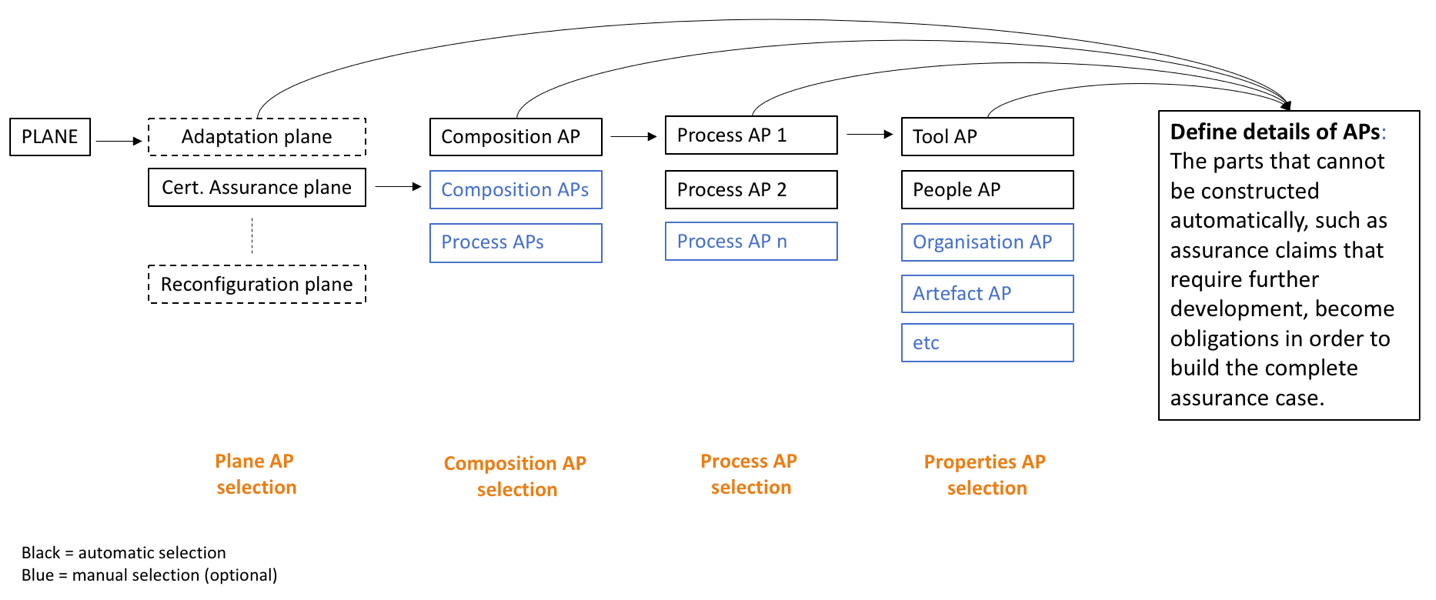
\includegraphics[width=.8\textwidth]{figures/automaticinstantiation.png}
\caption{\label{fig:automaticinstantiation2} Identification of patterns to be instantiated}
\end{center}
\end{figure}

\subsubsection{Automated Instantiation Based on the System Model}\label{sec:instantiation-systemmodel}
As opposed to using both the argument patterns and Adaptive MILS system model to construct the assurance case, another manner of establishing the assurance case may be by solely using the Adaptive MILS system model in the SLIM specification. The proposed way of achieving this is to specify the safety and/or security requirements, assumptions and evidence requirements in the Adaptive MILS system model directly. These requirements may be derived from regulatory standards or specified by the system owner. The specification of the various components and subcomponents of the system in the Adaptive MILS system model are taken to establish the structure of the assurance case. The advantage of this approach is that the arguments in the assurance case are completely tailored to a particular system, and do not have to be further refined subsequent to construction to the same extent as when generating an assurance case from a generic set of patterns. It has to be emphasised, however, that the safety and/or security requirements need to be carefully considered and specified in the Adaptive MILS system model and that any potential threats are identified and included when establishing the requirements in order to prevent confirmation bias. Taking a standards-based approach may aid in assuring all relevant security and safety claims, and assumptions are addressed for a particular type of system. 

\subsubsection{Modifications to the System and Maintaining the Assurance Case}\label{sec:modifications}
Whenever modifications to the overall system are required to satisfy the security or safety policy (as opposed to the transitions between internal pre-defined modes of compositions or components), the adaptation plane makes modifications to the current system model. It is envisioned that this occurs by establishing a new system model, which comprises the modification of components. The new system model is then directed to the configuration plane, where it is checked against local and system policies by the configuration state controller before instantiation. The configuration state controller permits or denies the new system model, based on the reconfiguration constraints (database). Afterwards, a new, or updated, assurance case may be generated. 

New assurance cases can be generated with the assistance of the AM-ETB, based on the current system model, upon request or at certain specified time intervals, rather than automatically generating new assurance cases each time the system changes. The advantage of generating assurance cases at certain intervals (for instance, daily or weekly) or upon request, is that computational overhead is kept to a minimum.  

Assurance cases are generated by establishing direct relationships between Adaptive MILS assurance case argument patterns and CITADEL system models, as described in Section~\ref{sec:automated-instantiation}. Taking this integrated approach to developing the Adaptive MILS assurance argument results in various advantages. First of all, it leads to improved change control for the assurance argument; changes to the system design are reflected in the argument. It additionally has the potential to automatically feed back the results of analysis of the assurance case into the development models \cite{D-MILS-D2.4}: "only once all the models impacted by the change have been updated can a new valid instantiation of the assurance argument be created" \cite{D-MILS-D2.4}. An assurance case argument is finished when the total number of nodes is the same as developed and instantiated nodes. Note that this does not guarantee the quality of the Adaptive MILS system; evidence is required to indicate the quality of the system.

\paragraph{Maintaining Assumptions}

Each assurance pattern has the possibility to include one or several assumptions, which can be added to any goal or strategy included in the assurance patterns. Whenever there is a modification to the system, the AM-ETB will automatically list assumptions that should be clarified or modified: "The problem in updating and maintaining safety/security assurance does not arise from the form of the assurance documentation or in updating the argument once the need for it is established, but in relating the assurance case to the detailed design decisions so that when a design is changed, it is possible to determine what assumptions in the safety analysis are involved" \cite{Weinstock07arguing-security}. Even though the AM-ETB will list which assumptions should be modified, the refinement of the assumptions are to be carried out manually. 

\newpage
\section{Assurance Cases for Other Domains}\label{sec:ac-other}
This portion of the report represents a new effort to develop assurance case strategies and corresponding assurance case argument patterns for the application of O-ETB to new domains, such as IoMT as envisioned by the MedSecurance project.

This section will be incrementally updated as the content is developed through collaborative efforts on the MedSecurance project use cases.

\subsection{IoMT}
\subsection{ISO 81001-2-1}
\cite{ISO-81001-2-1}

\subsection{MedSecurance Risk Based}



%%%%%%%%%%%%%%%%%%%%%%%%%%%%%%%%%%%%%%%%%%%%%%%%%%%%%%%%%%%%%%%%%%%%

\clearpage

% % % % % % % % % % % % % % % % % % % % % % % % % % % % % % % % % % % % % % % %
\addcontentsline{toc}{section}{References}

\bibliographystyle{plain}
\bibliography{References/d-mils+extra}
\clearpage

\end{document}

